
\section{Introduction}
\label{sec:org777ce67}

Once underway, a wide variety of people will have in interest in tracking the progress of Rubin Observatory in making the Legacy Survey of Space and Time (LSST).
In some cases, the interest is general, focused primarily on understanding whether the project is living up to expectations.
Many others will have more specific interests.
Scientists who will be using the data need to understand what data is currently available, plan for what will be available in the future, and provide informed suggestions and feedback to the survey project. 
Members of the project itself will need to be able to identify problems and opportunities early, and adjust the survey's observing strategy accordingly.

Several Rubin Observatory planning documents recognize this need, and include related requirements:
\begin{itemize}
\item \href{https://ls.st/lse-29}{LSE-29}, the "LSST System Requirements Document," requires that the project "provide periodic status reports on the progress of the survey to allow both operations staff and the community to assess the survey progress" (LSR-REQ-0065), "create the necessary survey performance evaluation tools to predict the final results of the ten year survey based on the actual survey completed to date, assess the impacts of survey strategy changes resulting from changes in scientific priorities, and support the planning of the survey on a variety of time scales, from nightly through the entire 10 year duration" (LSR-REQ-0066), and "monitor the scientific and technical progress of the survey, communicate with the scientific user community and establish survey priorities, and adjust the survey design as needed to accomplish its goals given these priorities and achieved performance" (LSR-REQ-0070). Furthermore, LSE-29 describes the role of an Observing Scientist who will need tools for oversight of the data collection process, including intervention in the normally autonomous operations process (LSR-REQ-0071).
\item \href{https://ls.st/lse-30}{LSE-30}, the "Observatory Systems Specifications," repeats the requirement that the project "provide the tools and administrative processes necessary to monitor the progress of the ongoing survey, provide reports on the progress of the survey, respond to feedback from the science community, and evaluate the impact of changing science priorities over the 10 year survey lifetime" (OSS-REQ-0033), and create summaries (OSS-REQ-131, OSS-REQ-0406), and publish visits ahead of observing them (OSS-REQ-0378). In addition, LSE-30 has several other requirements for monitoring that are of interest for scheduling and progress purposes (OSS-REQ-0056, 0067, 0068, 0072, 0078, 0079, 0314).
\item \href{https://ls.st/lse-369}{LSE-369}, the "LSST Scheduler Requirements" document, specifies several reporting requirements for the scheduler, including requiring that the scheduler "monitor the survey and produce daily summary reports, computing metrics for each science program" with automatically generated tables and plots (SCD-REQ-016); that the scheduler "publish the predicted schedule of visits right after the posting of the next target to the queue" (SCD-REQ-058); and that it "provide a set of indicators for reporting the progress on each science proposal and the overall survey, in the technical quantities that are part of the goals in its algorithms" (SCD-REQ-0059).
\item the \href{https://docushare.lsst.org/docushare/dsweb/Get/Document-36797/Rubin\%20Observatory\%20Operations\%20Plan\%20April\%202020.pdf}{Rubin Observatory Operations Plan} of April, 2020 states that the System Performance department will "Ensure that the observing strategy being implemented by the scheduler software is on track to achieve its science requirements at the end of 10 years. Achieving this goal will involve simulating the remaining survey time; folding in an evolving understanding of the Observatory system and ascertaining whether a change to the Scheduling algorithm or configuration may be warranted. In addition to meeting basic survey requirements, it may be possible to maximize the breadth of science that can be done with LSST by making minor changes to the observing strategy. The (internal) Survey Evaluation Working Group will include representation from Observatory Operations and Data Production, and will evaluate quarterly the current and expected performance of the survey and scheduler (as analyzed by the Survey Scheduling Team) and make recommendations to the Director on any needed tactical changes to the survey cadence (e.g., due to impact of weather, telescope or data processing responses to the schedule, etc)."
\end{itemize}

Although they emphasize the need for progress monitoring for strategy optimization and describe some reports in which such information is to be reported, they do not specify the specific data, metrics, or plots to be used for such monitoring or included in these reports.
The specific set of diagnostics will evolve over the course of the survey, but three sources can guide the generation of an initial set:
\begin{itemize}
\item The formal requirements on the survey, for example as specified by LSE-29.
\item Metrics proposed by science collaborations for evaluation of survey strategy.
\item The experiences of precursor surveys such as the Sloan Digital Sky Survey (SDSS), Dark Energy Survey (DES) and the Zwicky Transient Facility (ZTF), in so far as there are relevant similarities between the surveys. Such experience can be useful both in what was these groups felt they did well, and what they wished they had done but did not.
\end{itemize}

Progress and strategy diagnostics (metrics, plots, and other figures) are usefully characterized by several features:
\begin{description}
\item[{Audience}] Different diagnostics and figures are useful to different audiences. Possible audiences include reviewers for and administrators of funding agencies, Rubin Observatory management, LSST science collaboration scientists, the Rubin Observatory Observatory Scientist, Observatory Support Scientists, Observing Specialists, Scheduler Scientists and Survey Software Engineers, astronomers working on other projects, other members of the astronomical community, and the general public.
\item[{Format}] The diagnostics may take any of several forms, including simple scalars, time series and other plots, maps, or other representations of distributions.
\item[{Timing}] Diagnostics will need to be produced on range of timescales, ranging from hours to months. Some need to be produced shortly before or after each night of observing, or even periodically throughout the night. Others can be produced on a monthly schedule, or only in preparation for meetings and reviews.
\item[{Required data}] Data required to produce different diagnostics may originate in a variety of sources, including observatory telemetry, data products from Data Management, or sources outside the project (e.g., weather services).
\item[{Computing resources}] In some cases diagnostics can be produced with minimal calculation from available data sources. In other cases significant processing, up to and including suites of \texttt{opsim} simulations and corresponding calculation of metrics using \texttt{MAF}, will be required.
\end{description}

Each of these characteristics place requirements on the tools used to generate and provide access to the diagnostics.

\section{Use Cases}
\label{sec:orgeaeaad3}
\subsection{Pre-night review}
\label{sec:orgbffb978}

\begin{description}
\item[{Purpose}] To catch potential problems with the scheduler before the night begins, and to inform the expectations of the night staff (observing specialists) so that they know when intervention is needed, or when experts need to be called for assistance during the night.
\item[{Context}] Before each night of observing, a plan for the night needs to be created and reviewed, and the observatory staff needs to be briefed about the night to come. The person supervising scheduling for the night will complete this use case, generating the necessary simulations and corresponding diagnostics needed to find problems with the scheduler and brief the observing specialists. The plots and diagnostics produced will also be used by the observing specialists during the night as a reference in supervising the scheduler.
\item[{Primary actor}] The person supervising scheduling for a specific night. The Rubin Observatory Operations Plan (2020), suggests that this will be the observatory scientist, although an observatory support scientist or scheduler scientist also seem consistent with that plan.
\item[{Other stakeholders}] The observatory scientist, observatory support scientists, observing specialists, survey scheduling team, and sometimes the survey evaluation working group.
\item[{Trigger}] A set time in the afternoon before a scheduled night of observing.
\item[{Success conditions}] Observing specialists and other night staff are prepared for the night, with the information and resources necessary to distinguish acceptable scheduler behavior from behavior requiring intervention or assistance from experts.
\item[{Main success scenario}] On most nights of routine observing:
\begin{enumerate}
\item The scheduling supervisor for the night generates one or more simulated schedules for the night and a set of diagnostics on both the current state of the survey and the simulated schedules.
\item The scheduling supervisor verifies that the simulated schedules are appropriate for night, given the current state of the survey.
\item The scheduling supervisor uses the generated plots and other diagnostics to brief the observing specialists on the expected behavior of the scheduler during the night.
\item Observing proceeds, and the observing specialists verify that the scheduler is behaving according to expectations set in the briefing, using the generated plots and diagnostics as references.
\end{enumerate}
\item[{Variant scenarios}] The scheduling supervisor or observing specialists may detect anomalies or incorrect behavior in either steps 2 or 4. Further diagnostics and exploration may be required, but the specific requirements will vary considerably, and are outside the scope of this use case. Experts on the scheduling team may be contacted for assistance. Once any issues have been resolved, the set of night diagnostics may be regenerated for verification.
\end{description}

\subsection{Night Reports}
\label{sec:orge3c2faa}
\begin{description}
\item[{Purpose}] To alert the observatory scientists,  scheduling team, survey evaluation working group, and other experts on scheduling to potential problems requiring attention. To keep Rubin Observatory staff, science collaborations, and others interested in the state of Rubin Observatory and the progress on LSST up to date.\footnote{The night summaries have many purposes beyond these, beyond the scope of this document.}
\item[{Context}] At the end of each night, observatory staff will produce a summary of the night. Information on the progress of the survey during the night and diagnostics for the scheduler and related systems will be included in these summaries.
\item[{Primary actor}] The observing specialists on duty at the end of the night will be responsible for producing the night summary.
\item[{Other stakeholders}] All readers of the night summary, including but not limited to the observatory scientist and other staff, project management, subsystem specialists, data management staff, science working group members, and interested members of the general public.
\item[{Trigger}] The end of a night of observing.
\item[{Success conditions}] Any project members who might need to respond to events during the night have the resources needed to quickly and easily determine if their attention is required, and a starting point for doing so. Scientists interested in LSST data can quickly determine if data of interest to them was collected on the previous night. Management is aware of persistent night-time operations problems, and can direct resources accordingly. New observing specialists and others in training can get a sense of what current normal observing is like, and what they can expect, and current (already trained) observing staff is aware of any changes or problems they will need to look out for.
\item[{Main success scenario}] There are many variations on the "night summary" use case. A typical one would proceed as follows:
\begin{enumerate}
\item At the end of the night, the observing specialists generate a draft night summary using tools which mostly automate the process.
\item The observing specialists review the draft night summary, revising and providing text commentary when necessary.
\item The observing specialists make the night summary available (as a web page, on an RSS feed, by email, or by some other method).
\item In the morning, a scheduler scientist reviews the night summary, verifying that the scheduler behaved as expected, with the expected resulting data, and that other subsystems behaved as expected by the models used in the scheduler.
\end{enumerate}
\item[{Variant scenarios}] Different readers of the night summary will look for different kinds of information. Subsystems experts will follow up on any anomalies seen, usually with more general purpose tools. Data management staff will use information in the night summary to inform supervision of automated data processing, and prevent or resolve any problems the might occur while reducing the data. Many others may simply read the night summary to keep current on how the observing is going, and so the night summary becomes a mechanism for maintaining interest. Regularly updated and accessible progress plots are particularly valuable for helping collaborators and potential collaborators remain engaged.
\item[{References}] \begin{itemize}
\item Requirements documents LSE-30 and LSE-61 specify that a night report be produced (OSS-REQ-0131, OSS-REQ-0406, DMS-REQ-0394) within 4 hours (DMS-REQ-0096) and contain metrics on observatory performance (OSS-REQ-0131) and DM measured metadata about the data (DMS-REQ-0097), calibration (DMS-REQ-0101), and processing (DMS-REQ-0099), and include (unspecified) per-subsystem performance (OSS-REQ-0406).
\item Technical notes SQR-23: "Design of the notebook-based report system," and SQR-26: "Periodic report generation and publication via notebook templates" describe a jupyter notebook template-based system for generating night reports using a combination of data management and SQuaRE infrastructure.
\end{itemize}
\end{description}
\subsection{Survey Progress Reports}
\label{sec:org6e54112}
\begin{description}
\item[{Purpose}] To communicate the current survey progress to Rubin Observatory management, the science collaborations and other members of the astronomical community. To convey an understanding of the reasons for deviation from expected progress, and the long term impact of unexpected events and changes in plans to expectations of future progress and the final state of the survey. Data and presentation should be sufficient to elicit informed survey strategy related feedback and recommendations from the scientific community, and direction from the survey evaluation working group (SEWG), survey cadence optimization committee (SCOC), and other elements of Rubin Observatory management.
\item[{Context}] Each quarter (according to the 2020 Rubin Operations Plan), the observatory support scientists will produce a report presenting and discussing the current progress on the survey, and any revised expectations of future progress.
\item[{Primary actor}] The observatory support scientists.
\item[{Other stakeholders}] Rubin Observatory management, scheduler scientists, survey evaluation working group (SEWG), survey cadence optimization committee (SCOC), and science collaborations.
\item[{Trigger}] Calendar date (quarterly).
\item[{Success conditions}] Observatory management has an overall understanding of the state of the survey sufficient to direct resources and report to funding agencies. The science collaborations have the data and analysis needed to provide informed feedback and suggestions to the project. The survey evaluation working group (SEWG) and survey cadence optimization committee (SCOC) have the data and explanations they need to identify needed changes and evaluate changes to survey strategy.
\item[{Main success scenario}] In the primary success scenario, under which the survey has progressed roughly according to the expectations of the observatory support scientists and scheduling team:
\begin{enumerate}
\item Near the end of a quarter, an observatory support scientists collect the latest plots and diagnostics describing the state of the survey, and compiles them into a document with accompanying text describing how the achieved weather conditions (seeing, weather, atmospheric extinction) compared with expectations for the site, how instrumental and procedural performance compared with expectations, and the impact of any differences on survey progress. They also include the results of simulations starting with the current state and extending through the end of the survey.
\item The scheduling scientists review the draft report, and supplement it with additional plots or commentary if necessary.
\item The completed report is distributed to Rubin Observatory management, survey evaluation working group (SEWG), survey cadence optimization committee (SCOC), and science collaborations.
\item Science collaborations review the report, and prepare responses, if necessary.[fn: The procedure for submitting, evaluating, and responding to such responses is beyond the scope of this document, but the quality of the progress reports will drive the quality of these responses.]
\end{enumerate}
\item[{Variant scenarios}] Significant deviations from expected progress will result in a variety of different sequences, depending on the details of the deviations. For example:
\begin{description}
\item[{poor weather}] If the quarter had a month of particularly poor weather, such that the last month passed without collection of any useful data, scenario might proceed as follows:
\begin{enumerate}
\item The initial compilation and distribution of the draft proceeds as described in the main scenario steps 1 through 3, except for the addition of additional discussion related to the weather, and independent evaluation of the parts of the quarter in which the weather was more normal (to verify that other problems did not also contribute to the lack of progress). Differences between the previous and current project progress will be called out in the discussion.
\item Science collaborations propose changes in response to the unexpected lack of progress. For example, if the month of poor weather occurred near the end of a DDF season, some science collaborations interested in the DDF may wish to propose that the remaining DDF visits in the season be replaced by denser coverage of DDFs in later seasons, because any additional DDFs in the current season would be too isolated in time to be scientifically useful.
\end{enumerate}
\item[{under-performing filter}] Consider a case in which the visits from one filter have been shallower than expected, with the result that the accumulated number of exposures in each filter is as expected, but the accumulated co-added depth is shallower than expected.
\begin{enumerate}
\item The initial compilation and distribution of the draft proceeds as described in the main scenario steps 1 through 3, except for the addition of additional discussion related to factors affecting visit depth in the lagging filter, including clouds, sky brightness, and seeing at the times during which the images were taken and inferred throughput of the instrument, together with inferences concerning whether these conditions are likely to continue into the future. For example, z and y band might lag if the seeing happened to have been unusually poor during bright time, but seeing is not expected to correlate with the moon long term except by coincidence, so if this were the cause it would be unlikely to continue into the future. On the other hand, if the sky brightness in these filters were consistently significantly brighter than the model, then this would indicate a problem with the model, and one might infer that these filters would continue to fall further behind. In any case, the authors of the report would discuss the long term impact of the lagging filter, including final co-add depth, detection efficiency for different transients, and progress as measured in other science metrics, in both the long and short term.
\item The science collaborations review the report, and decide whether alterations in strategy might be required to mitigate its effects. For example, if an under-performing z band were found to be the limiting factor in photometric redshift measurements, and r and i band getting deeper visits than expected, the photometric redshift working group may propose changing the balance between numbers of visits in the different bands, replacing r and i band visits with z band visits. The plots and metrics in the report should support estimation of how many visits would have to be moved from r and i to z, and what impact this might have on final co-add depth.
\end{enumerate}
\end{description}
\item[{References}] \begin{description}
\item[{OSS-REQ-0033}] "The LSST shall provide the tools and administrative processes necessary to monitor the progress of the ongoing survey, provide reports on the progress of the survey, respond to feedback from the science community, and evaluate the impact of changing science priorities over the 10 year survey lifetime."
\item[{LSR-REQ-0070}] "The Observatory shall have the ability to provide periodic status reports on the progress of the survey to allow both operations staff and the community to assess the survey progress."
\item[{LSR-REQ-0066}] "The Project shall create the necessary survey performance evaluation tools to predict the final results of the ten year survey based on the actual survey completed to date, assess the impacts of survey strategy changes resulting from changes in scientific priorities, and support the planning of the survey on a variety of time scales, from nightly through the entire 10 year duration."
\item[{LPM-73 8.3.3}] specifies that science operations staff "measure progress against the survey plan. A written monthly progress report will be provided to Headquarters, and weekly updates will be tracked in Chile. Adjustments to the short term observing plan (choice of filters, relative priority of science programs, etc.)  will be made in Chile. If major changes to observing strategy appear to be required, Headquarters will ask the PST for recommendations."
\item[{2020 Rubin Operations Plan}] lists, as a duty of the observatory support scientists (section 13.2), "Responsible for producing a quarterly report on the scheduled/expected observations versus the performed observations. This analysis includes monitoring the assumptions used by the scheduler including slew times, shutter open/close times, readout times etc."
\end{description}
\end{description}
\subsection{Science project planning (static)}
\label{sec:orgae6075c}
\begin{description}
\item[{Purpose}] To determine when (or if) survey co-add data will be useful for a science project requiring a certain area at a certain depth.
\item[{Context}] A small group of astronomers comes up with a brilliant idea for a project, and conclude that they need a survey that covers at least 10000 square degrees and has \(5-\sigma\) limiting magnitudes of at least 26.0 in r and 25.0 in z. They want to know when Rubin Observatory might have collected the necessary data to construct such co-adds.
\item[{Primary actor}] Astronomers planning a project.
\item[{Trigger}] A group of astronomers has an inspiration for a project.
\item[{Success conditions}] The collaboration of astronomers has a good understanding of when their project will become feasible, or to what degree.
\item[{Main success scenario}] The group might take the following steps:
\begin{enumerate}
\item The astronomers retrieve plots of \(t_{\mbox{\tiny eff}}\) vs. calendar date for the filters for relevance from a recent night report or quarterly report.
\item They note that in most years, the slope of accumulated \(t_{\mbox{\tiny eff}}\) followed the baseline, but there was one year during which progress was more shallow, after which it returned to the nominal slope.
\item They estimate the date on which the \(t_{\mbox{\tiny eff}}\) corresponds to the magnitudes of interest for each filter, extrapolating from the latest point by eye, using the typical slope. They also use the maximum and minimum slopes (visually obvious from inspection of the plot) to estimate optimistic and pessimistic dates on which the data might have been collected.
\end{enumerate}
\end{description}
\subsection{Deep Drilling Field scheduler evaluation}
\label{sec:orge4cc32b}
\begin{description}
\item[{Purpose}] To evaluate the scheduler's performance in scheduling DDF fields.
\item[{Context}] The Deep Drilling Fields (DDFs) mini-survey consists of a set of additional visits at a handful of pointings. These additional visits will result in a denser cadence at the selected pointings, enabling the study of variable and transient objects over longer seasons and with a denser cadence. Furthermore, these additional visits will result in a much deeper co-add limiting magnitude for the limited area they cover. The success of the deep drilling mini-survey depends on the observing cadence, season length, and overall depths in these fields. Additionally, optimization of the DDF mini-survey depends on the same kinds of features all exposures do, including observation close to transit and when the sky brightness is as low as possible given restrictions imposed by the required cadence.
\item[{Primary actor}] The observatory support scientists and the scheduling team will both evaluate the scheduler's performance on DDF fields on a routine basis.
\item[{Trigger}] Evaluation of DDF scheduler performance may be triggered by any of several conditions, including:
\begin{itemize}
\item preparation for the pre-night review, during which the predicted DDF visits generated by the simulator require sanity checking.
\item preparation of night reports, so that the performance of the scheduler on DDF fields during the just completed night can be checked.
\item evaluation of scheduler changes, particularly proposed changes to DDF scheduler strategy.
\item preparation of survey progress reports. The DDF program is important for the success of LSST as a whole, and evaluation of progress observing DDFs should be included in the global progress reports.
\end{itemize}
\item[{Success conditions}] If successful, the actors in this use cases will be able to tell whether DDF fields were scheduled at appropriate times, including identifying nights when they should have been scheduled by were not, nights when they should not have been scheduled by were, and nights during which visits on DDF fields were scheduled at a different time than optimal.
\item[{Main success scenario}] The agent will need to produce and examine a collection of different diagnostics, including:
\begin{itemize}
\item a cadence plot, showing the nights on which each DDF field was observed, and the depths of the images obtained. Figure \ref{fig:org2e88796} shows a sample cadence plot.
\item a time use hourglass plot, showing the nights on which each DDF field was observed, and the time it was observed relative to transit. Figure \ref{fig:org1a3263e} shows an example time use hourglass plot.
\item rule-based condition checks. Several sciences collaborations have requested rule-based DDF strategies (e.g. each DDF field should be observed on a cadence of X days and a season length of Y days, at a minimum). Reports should flag any nights on which the rules adopted by the project are violated.
\item metric based checks. When triggered by new strategies or creation of global reports, the values of science metrics on each DDF field should be reported. For evaluation of DDF scheduling for individual nights (including the pre-night review and night reports), science metrics may be evaluated on simulations with and without DDF visits, and the effects on final science metrics and fraction of time taken by DDFs evaluated.
\end{itemize}
\end{description}
\subsection{Other Mini-survey evaluation}
\label{sec:orgf6505be}
\begin{description}
\item[{Purpose}] To estimate the effectiveness of an ongoing target of opportunity program (or other mini-survey), and its impact on the progress made on WFD science goals and other mini-surveys.
\item[{Context}] Current plans dedicate a fraction of Rubin Observatory observing time to mini-surveys. Estimation of the impact of these surveys on the WFD and other programs will not always be straightforward: visits scheduled for them will often also contribute to WFD goals, so even though the time taken for them may not be fully optimal for WFD science, it is not fully lost to it either. Furthermore, the effectiveness of the mini-survey must itself be evaluated for how well it progressing towards its own scientific goals. If it is making little progress but having a significant impact on WFD progress, the mini-survey observing strategy may need to be modified, or the mini-survey discontinued.
\item[{Primary actor}] the survey cadence optimization committee (SCOC)
\item[{Trigger}] Regular meeting of the SCOC.
\item[{Success conditions}] The SCOC has the data necessary to make informed decisions on renewing mini-surveys.
\item[{Main success scenario}] \begin{enumerate}
\item The SCOC examines the most recent survey progress report and reports from the science collaborations on status of the science from the mini-survey.
\item By comparing WFD science metrics actually achieved to those that opsim simulations report would have happened had the mini-survey not taken place, the SCOC determines whether the mini-survey's impact on the FWD was well estimated, or if it was more or less disruptive than expected.
\item The SCOC recommends the continuance, alteration, or conclusion of the mini-survey. For example, it may apply additional conditions on a target of opportunity mini-survey if triggered visits were less useful for the FWD than had been expected. Alternately, if a mini-survey has been under-performing on its own scientific metrics, but alterations to survey strategy have had little or no impact on WFD science goals, the SCOC may recommend that the mini-survey be expanded.
\end{enumerate}
\end{description}
\section{Metrics, plots, and other diagnostics}
\label{sec:org922c37a}
\subsection{Survey state descriptions}
\label{sec:org3a7f0df}
Figures and diagrams describing the current "state of the survey" will be of great interest to the community as a whole, and providing an understanding of whether they correspond to the plan for the survey will be essential for explaining how well the survey is proceeding.
Examples of such diagrams will include:

\begin{description}
\item[{depth maps}] Maps of the survey showing the numbers of total visits, numbers of visits in each filter, and co-add limiting magnitude in each filter are likely to be the most prominent figures that show the current state of the survey. Current tools for evaluation of survey simulations produce examples of such plots, and \href{http://astro-lsst-01.astro.washington.edu:8081/allMetricResults?runId=392\#Basic\%20Maps}{results pages} show examples of such maps for the end of simulated surveys. Maps cut in an assortment of ways, for example including only visits with PSF widths narrower than some cutoff, may also be of interest. Figure \ref{fig:org11f36cc} shows an example of a depth map produced by MAF, for the end of a baseline survey.
\item[{depth/area plot}] A plot of the total area on the sky covered by the survey as a function of minimum depth will also be a useful representation of progress. Figure \ref{fig:org548d841} shows an example of such a plot produced by MAF, for the end of a baseline survey. When used to show survey progress, reference curves from a baseline simulation should be included as well.
\item[{filter use hourglass plots}] A single graphic that shows the distribution of filter use by time of night and year, and in relation to the moon, can indicate whether dark time is being used efficiently. The \href{http://astro-lsst-01.astro.washington.edu:8081/allMetricResults?runId=392\#Hourglass}{results pages} give examples of such plots for the ends of simulated surveys. Figure \ref{fig:orgc770d9a} shows an example of such a plot produced by MAF, for the end of a baseline survey.
\item[{time use hourglass plots}] A single graphic that summarizes how time has been used by the survey so far will also be of wide interest. A plot will be a similar appearance to that of filter use hourglass plots, and like the plot will indicate time of year on one spatial axis and time of night on the other. Instead of indicating filter, however, this hourglass plot would indicate whether the pointing being observed corresponds to the FWD survey, a mini survey, or (if not science observing) what other activity was taking place. Likely categories to by symbolized by colors include: downtime due to equipment failure, downtime due to regular maintenance or engineering, time closed due weather, time open and observing but without useful exposures (e.g. due to thick clouds), time spent on observations outside the WFD footprint (possibly separated by mini-survey), time spent on DDFs, and other time in the WFD. Figure \ref{fig:org1a3263e}indicates what such a plot might look like, showing time spent on DDF fields and FWD fields with and without bluer filters. A production version of this plot could also indicate downtime from weather, engineering time, or equipment failure.
\item[{data quality hourglass plots}] A plot similar to the filter and time use hourglass plots, but uses the color coding to represent data quality (as measured by \(5\sigma\) limiting magnitude relative to nominal depth or \(t_{\mbox{\tiny eff}}\)\footnote{\(t_{\mbox{\tiny eff}} \equiv 10^{\frac{4}{5}(m_{\mbox{\tiny lim}} - m_{0})}\), where \(m_{0}\) is some reference limiting magnitude. \(t_{\mbox{\tiny eff}}\) has two advantages over the more traditional limiting magnitude: first, it scales linearly with time under similar conditions, and second, it is additive under coaddition.}). Figure \ref{fig:orgbe6638e} shows an example of such an hourglass plot. Note that the seasonal variation and variation with moon phase are immediately apparent.
\item[{transient detection efficiency maps}] Maps of detection efficiency for different classes of variable objects (bright and faint near Earth objects (NEOs), TransNeptunian Objects (TNOs), Tidal Disruption Events (TDEs), fast microlensing events, type 1a supernovae, and others) over the footprint, for the entire survey so far and for the current season.\footnote{Gaps between seasons may be defined to be gaps between visits than include the date on which the sun has the same R.A. as the point on the sky.}
\item[{deep drilling field (DDF) cadence plots}] A set of plots (one for each DDF) showing the nights on which each DDF has been observed in the current season, and marking the time since it was last observed in each filter. Such plots may also encode the depth of exposures in each band on each night. Figure \ref{fig:org2e88796} shows a sample cadence plot made using simulated data.
\item[{DDF transient efficiency plots}] The detection efficiency and actual numbers of detections for different classes of transients may be plotted as a function of date for each DDF. If these plots were combined with the DDF cadence plots, these plots may also guide an intuition for how gaps of different sizes affect the science for different classes of objects.
\end{description}

\begin{figure}[htbp]
\centering
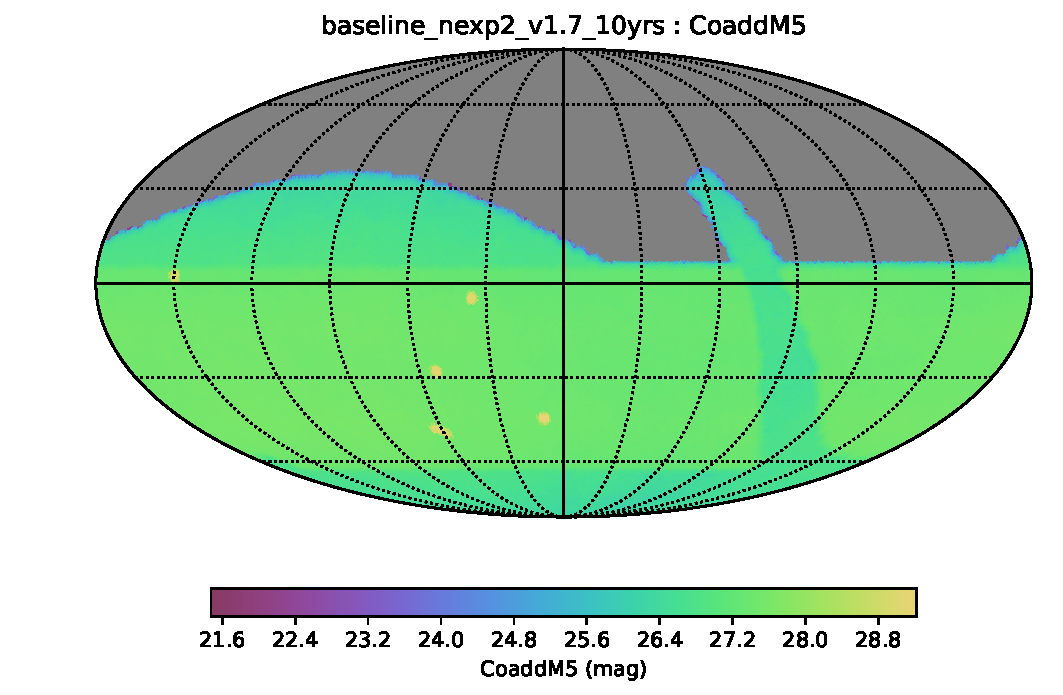
\includegraphics[width=.9\linewidth]{./figures/baseline_nexp2_v1_7_10yrs_CoaddM5_HEAL_SkyMap.pdf}
\caption{\label{fig:org11f36cc}Example depth map from MAF, for the state of the survey at the conclusion of the 10 year baseline simulation.}
\end{figure}

\begin{figure}[htbp]
\centering
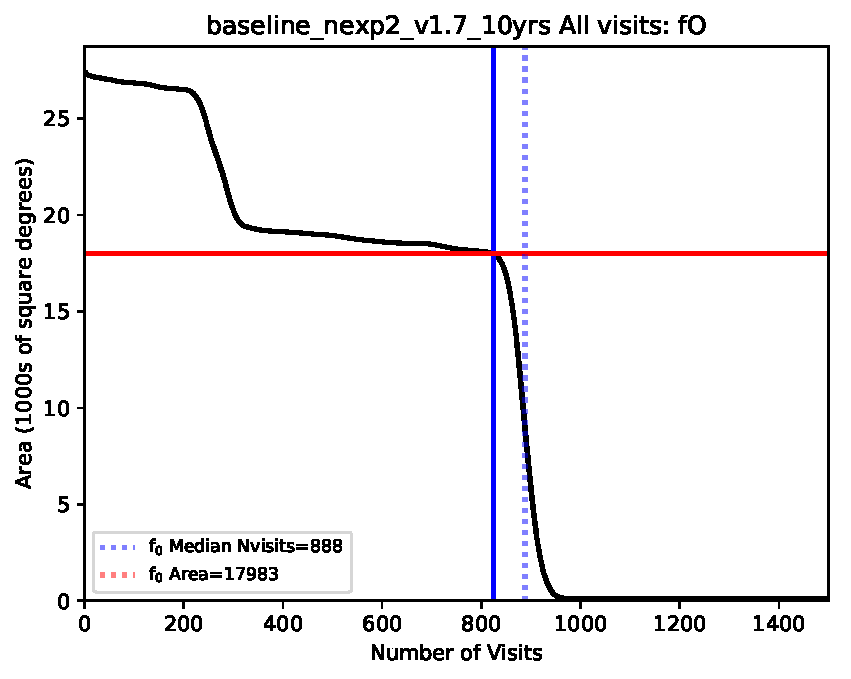
\includegraphics[height=0.4\textheight]{./figures/baseline_nexp2_v1_7_10yrs_fO_All_visits_HEAL_FO.pdf}
\caption{\label{fig:org548d841}Example depth-area plot from MAF, for the state of the survey at the conclusion of the 10 year baseline simulation.}
\end{figure}


\begin{figure}[htbp]
\centering
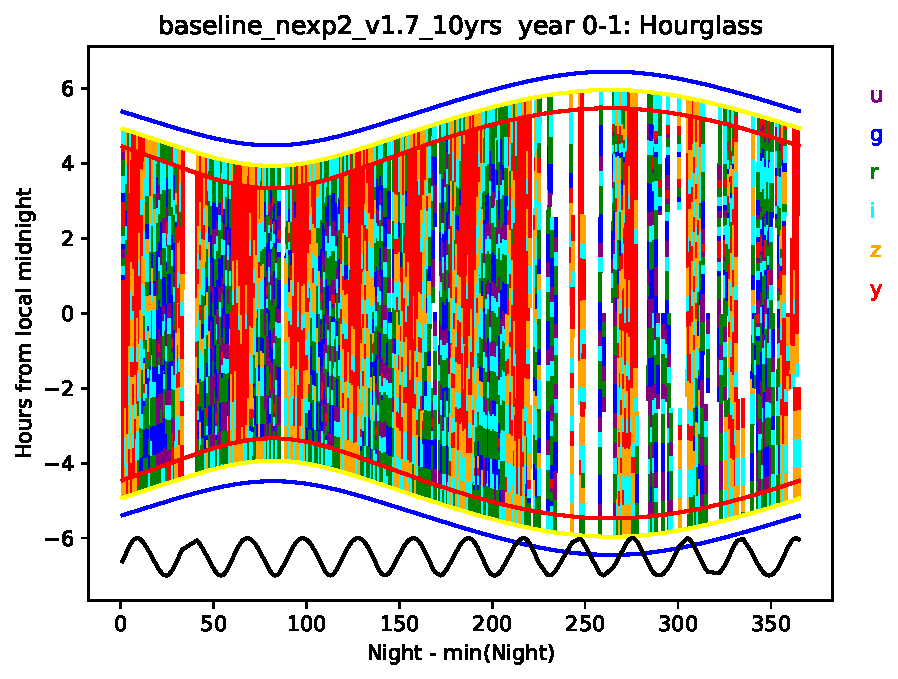
\includegraphics[height=0.4\textheight]{./figures/baseline_nexp2_v1_7_10yrs_Hourglass_year_0-1_HOUR_Hourglass.pdf}
\caption{\label{fig:orgc770d9a}Example filter use hourglass plot from MAF, for the state of the survey at the conclusion of the 10 year baseline simulation. The black line along the bottom shows the lunar phase. The red and blue lines show nautical and civil twilight.}
\end{figure}

\begin{figure}[htbp]
\centering
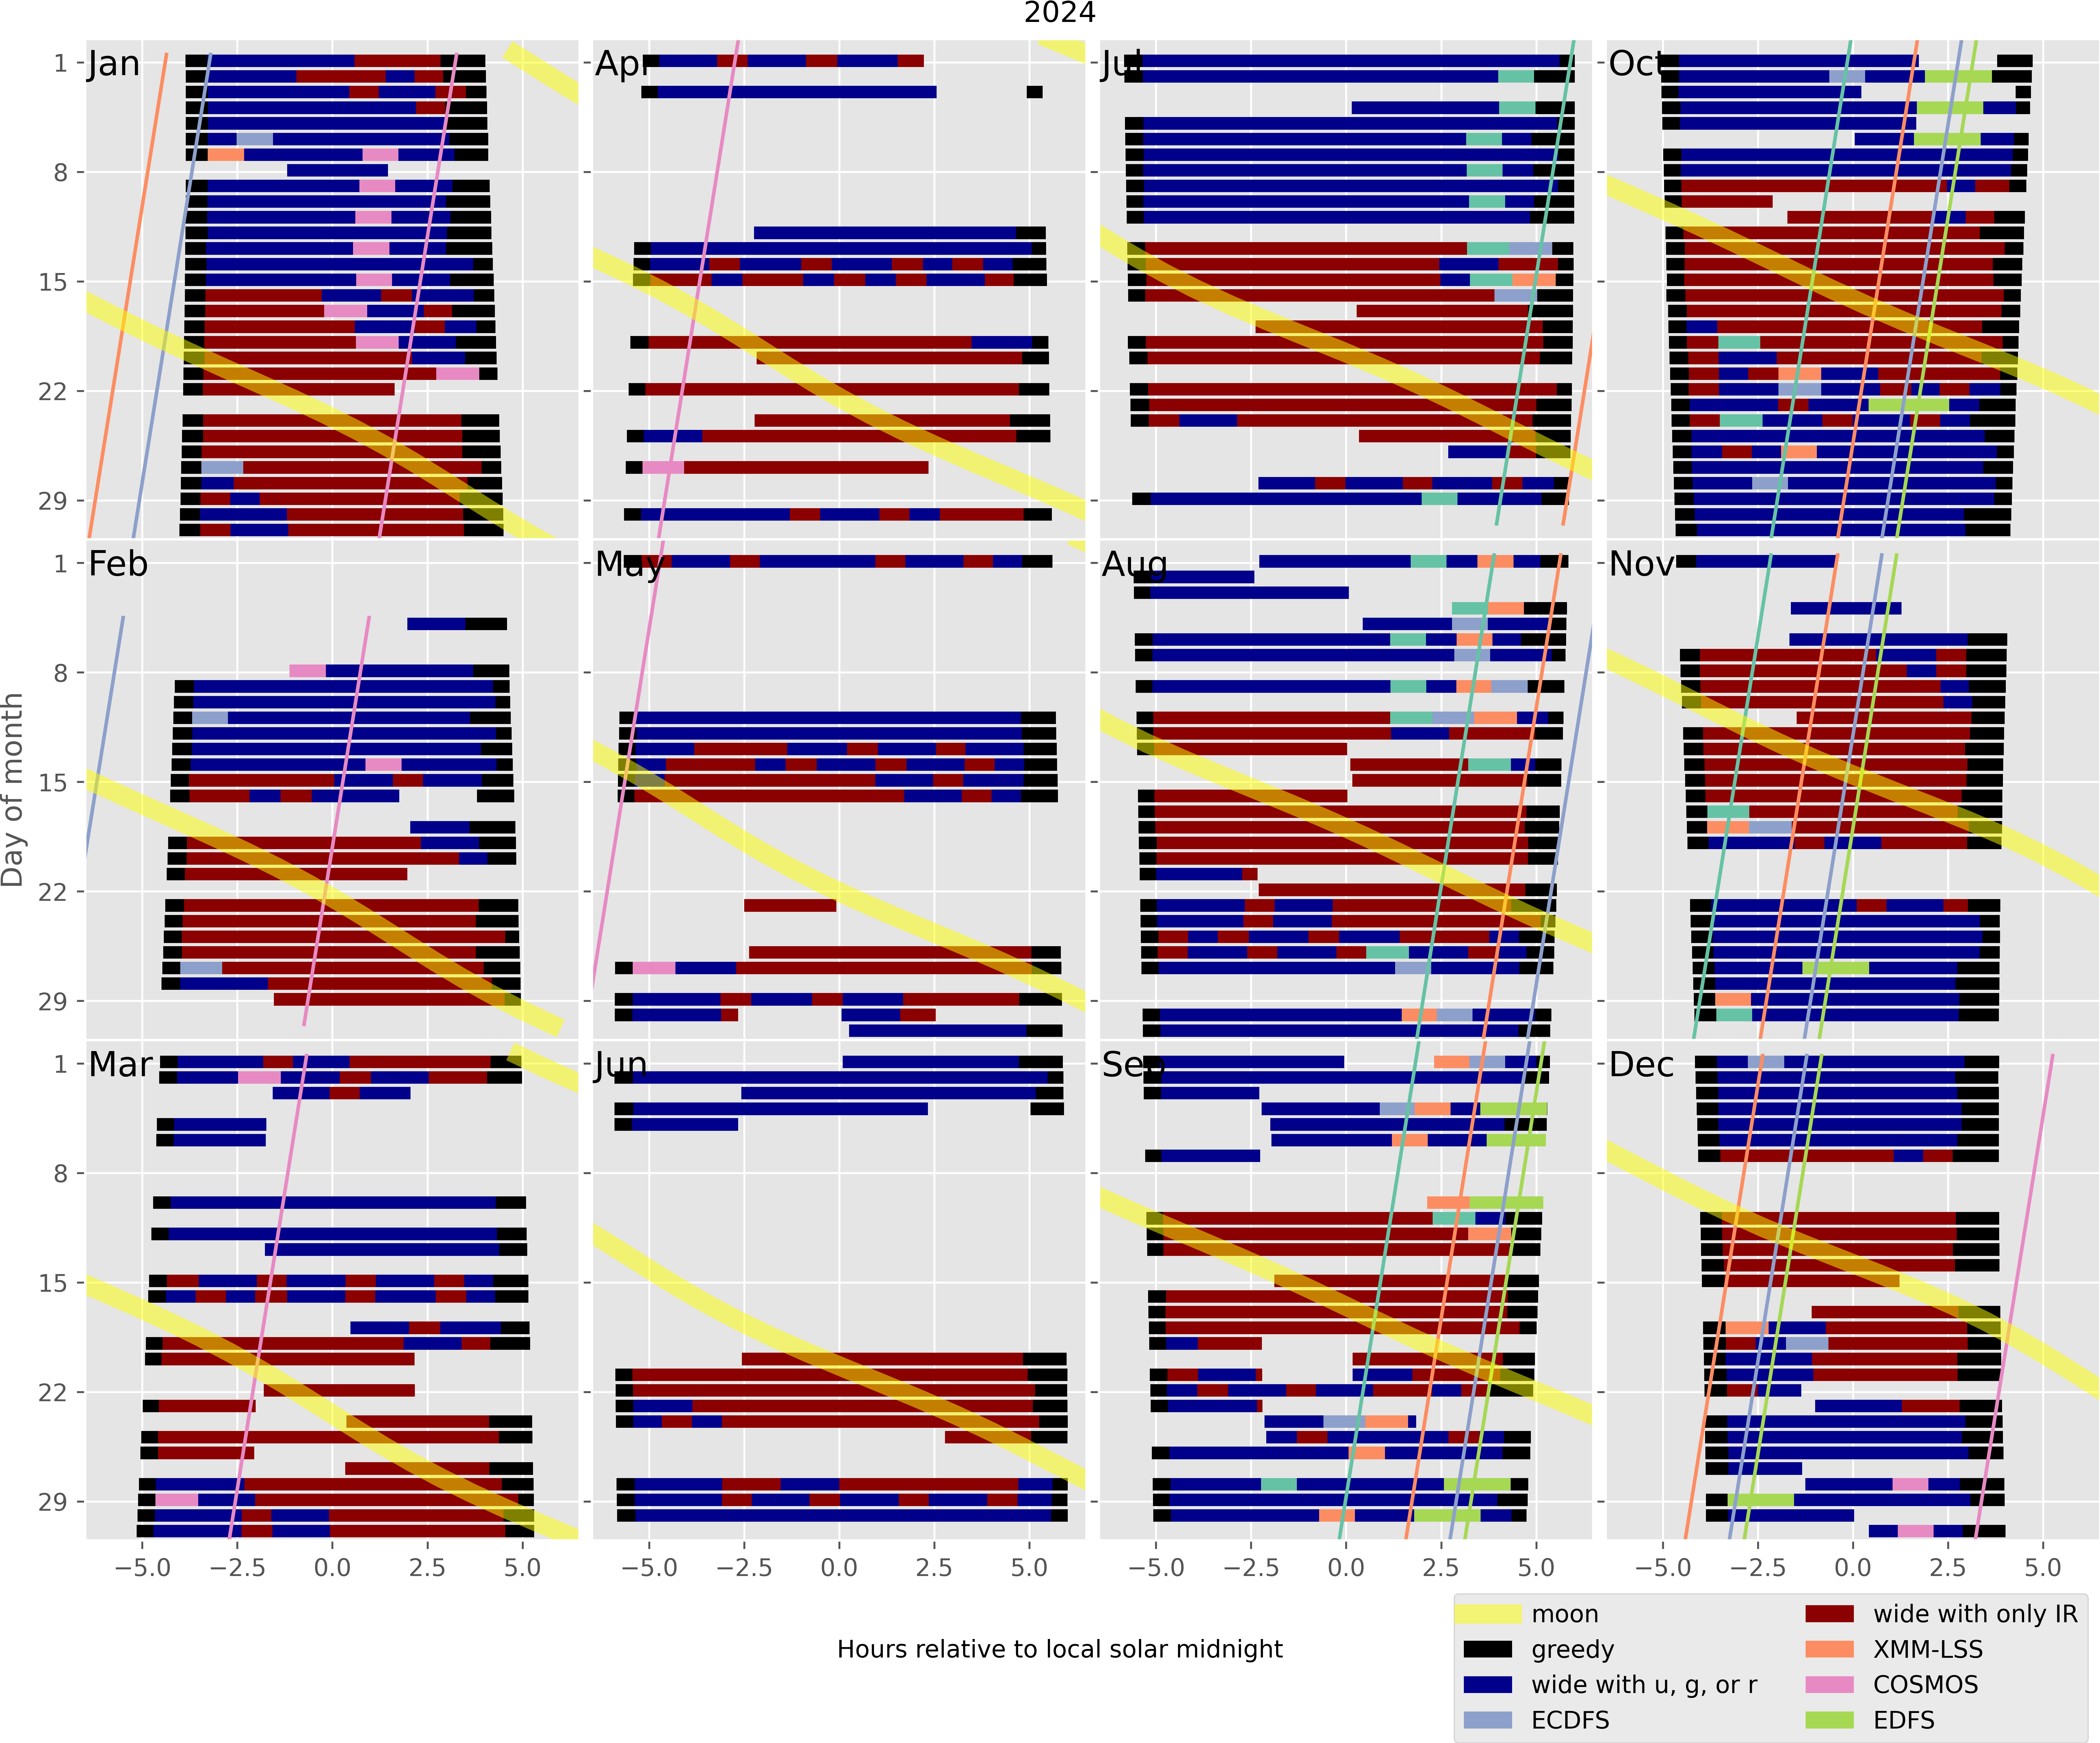
\includegraphics[width=1.0\textwidth]{./figures/block_hourglass.png}
\caption{\label{fig:org1a3263e}Example time use hourglass plot, for one year of the 10 year baseline simulation. The gray and black background shading mark civil, nautical, and astronomical twilight times, and full dark. Orange bars mark times of night when `opsim` is selecting visits using the "greedy" algorithm. Red bars marks times when `opsim` scheduled wide-survey blocks that include only IR filters (i, z, and y), while blue bars mark wide survey blocks with at least some u, g, or r visits. Horizontal bars of other colors mark different DDF fields. Slanted vertical lines mark transit times for each DDF field: if a DDF field is observed as it transits, the slanted vertical line passes through the horizontal bar of the same color. The thick yellow line marks the transit time of the moon, and the dotted yellow lines mare the moon's rise and set time. The moon is full when it transits at midnight, so the time the yellow line crosses the horizontal bar for the date indirectly indicates the phase of the moon. Note that the horizontal red bars surround the yellow line, indicating that the scheduler is correctly scheduling filters with the IR filters when the sky is bright.}
\end{figure}

\begin{figure}[htbp]
\centering
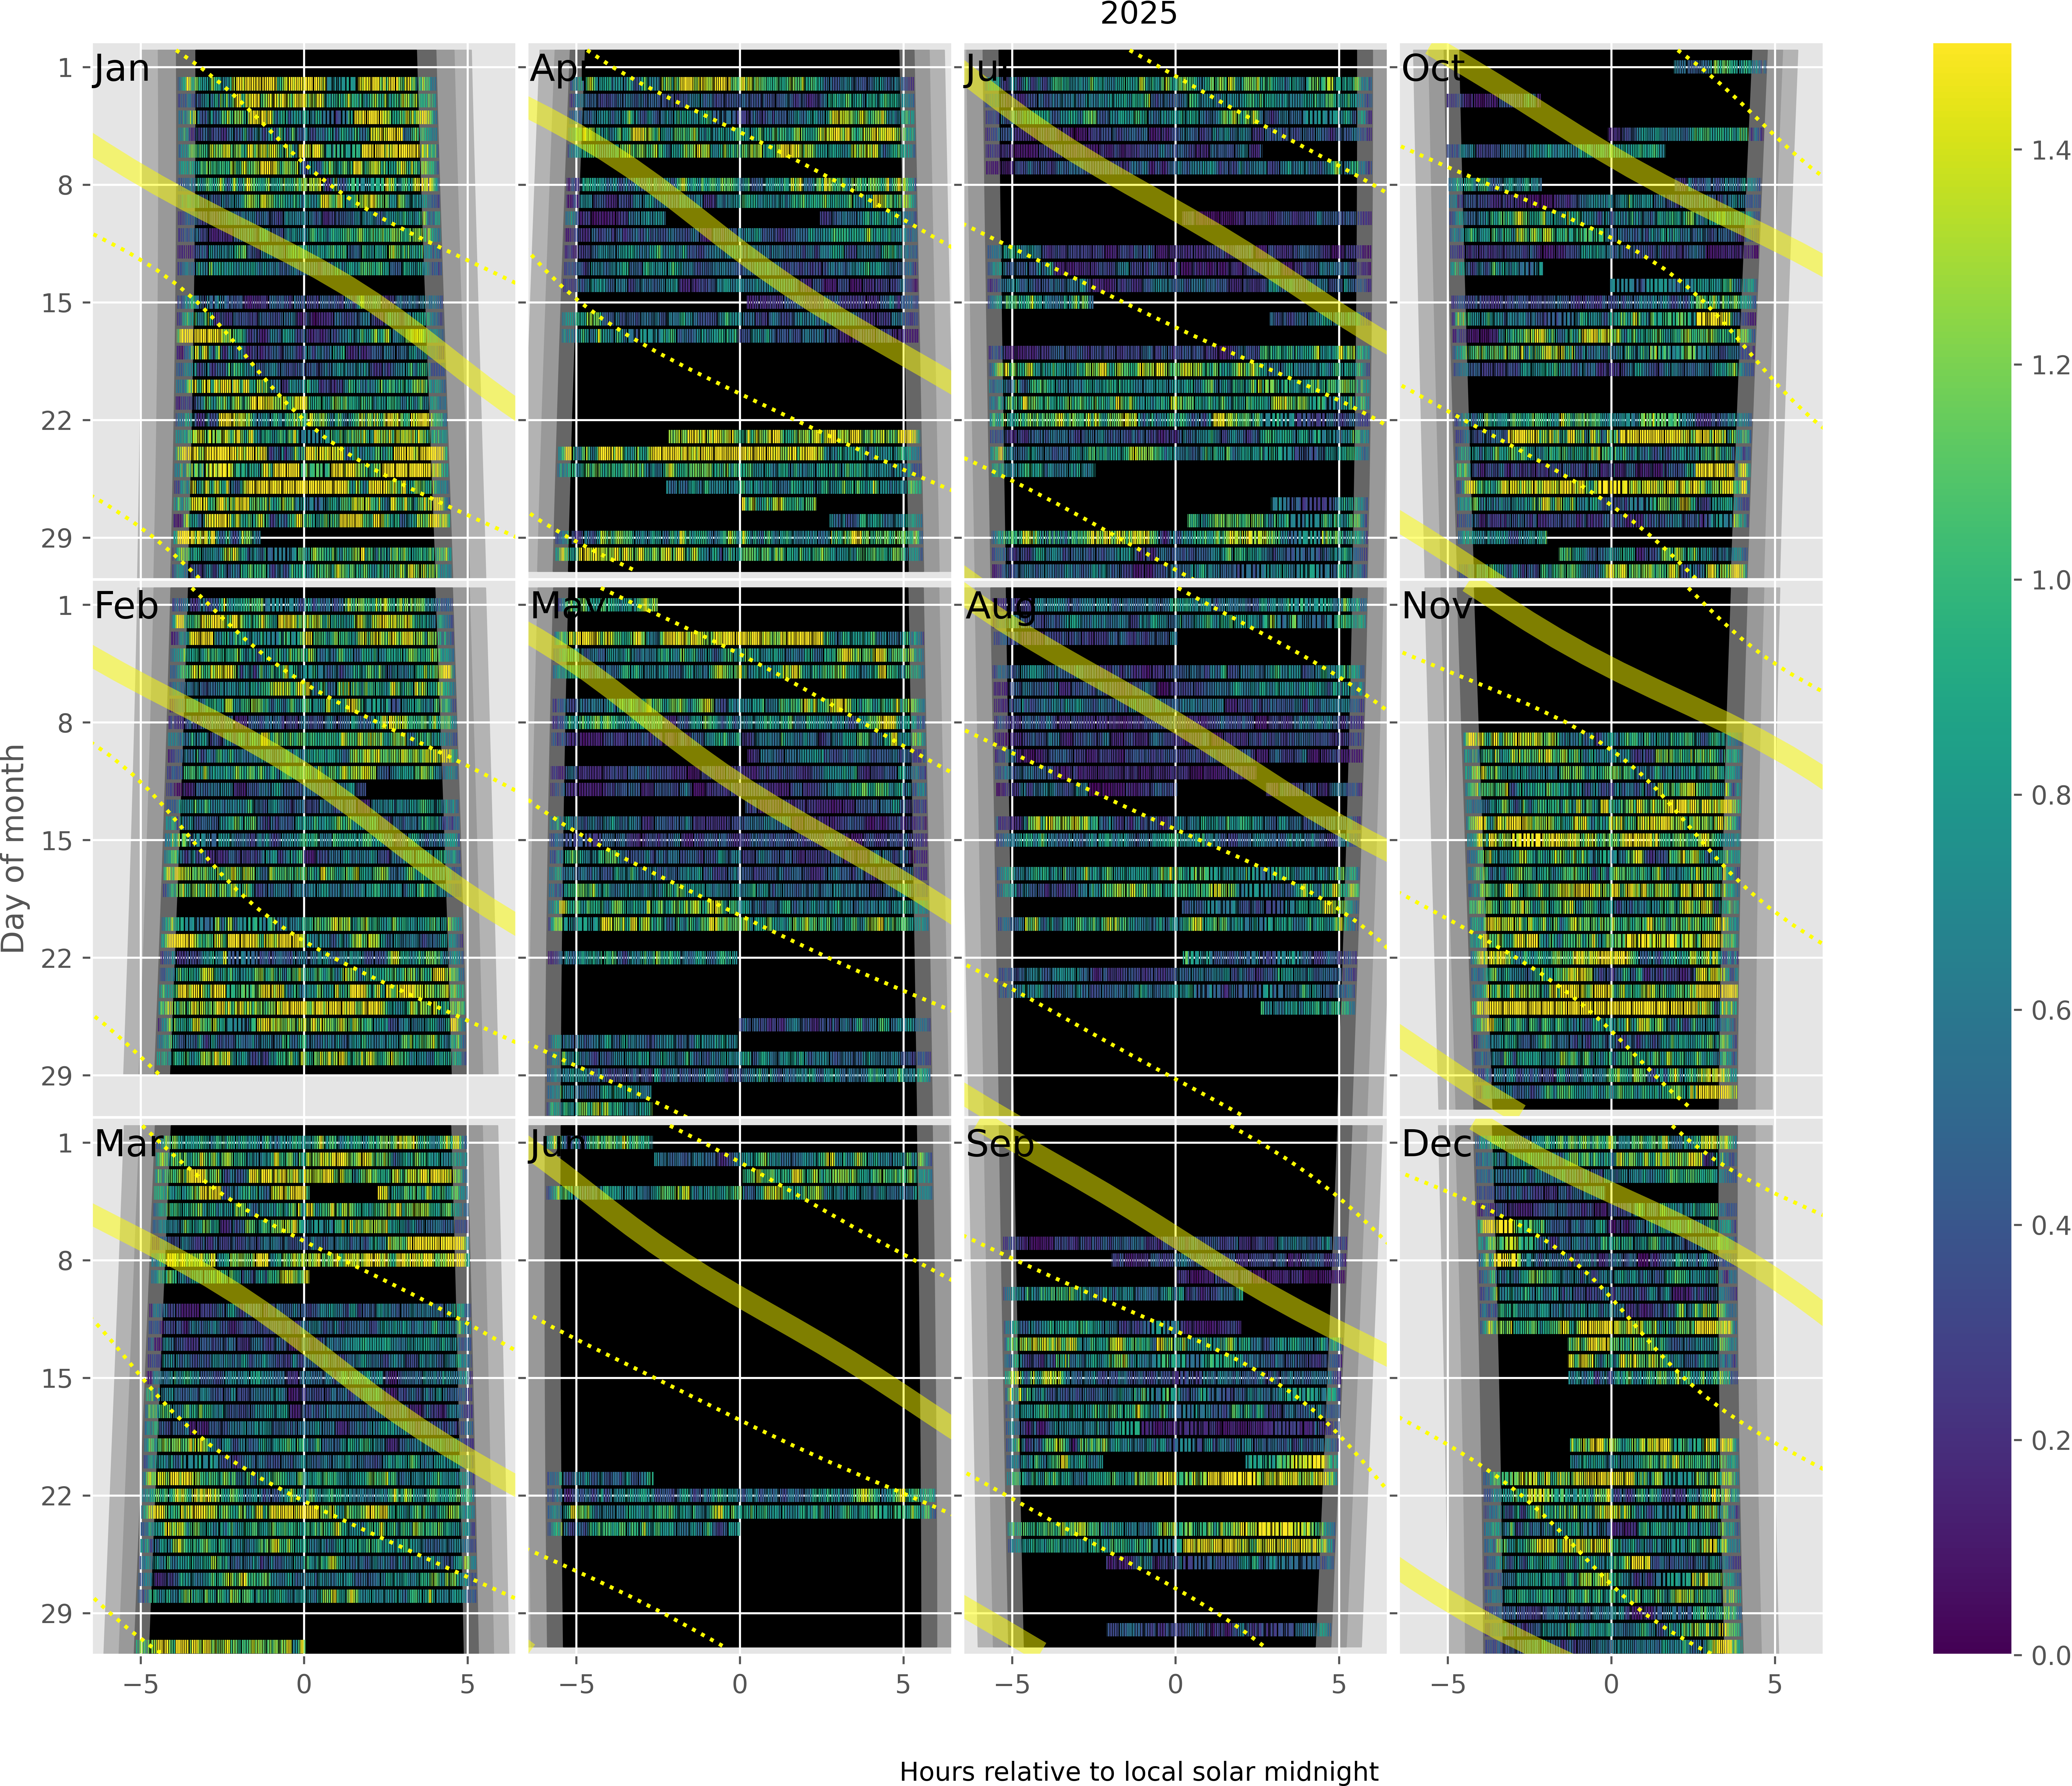
\includegraphics[width=1.0\textwidth]{./figures/teff_hourglass.png}
\caption{\label{fig:orgbe6638e}Example data quality hourglass plot, for one year of the 10 year baseline simulation. The gray and black background shading mark civil, nautical, and astronomical twilight times, and full dark. The thick yellow lines mark the transit of the moon, and the dotted lines, the lunar rise and set times. Colors mark the \(t_{\mbox{\tiny eff}}\) of visits taken at the given time.}
\end{figure}


\begin{figure}[htbp]
\centering
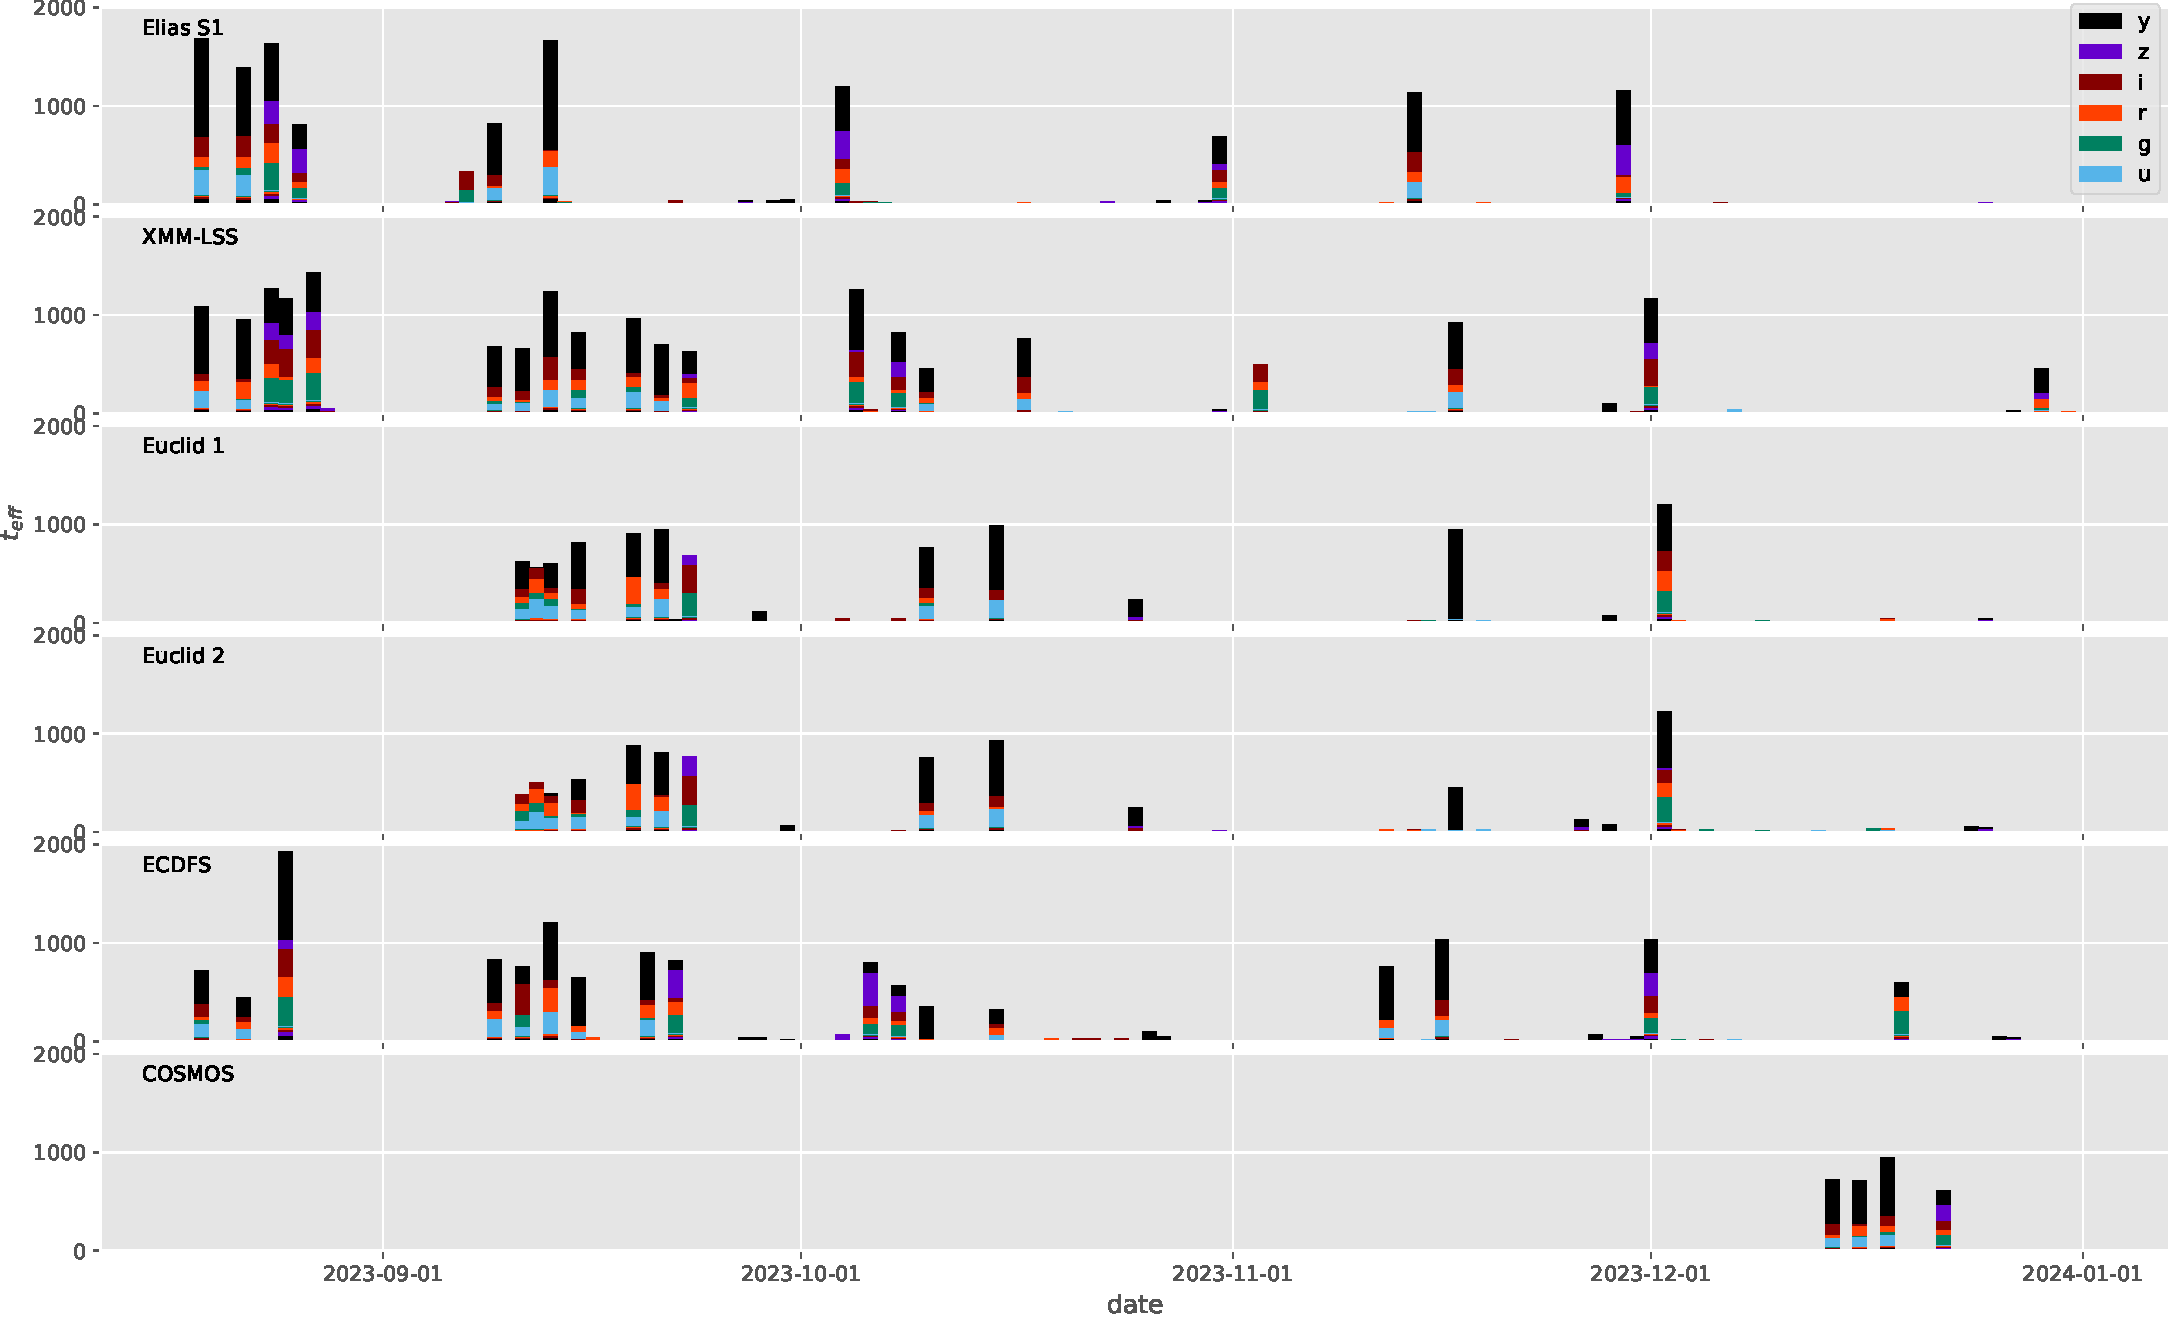
\includegraphics[height=0.4\textheight]{./figures/snhistory.pdf}
\caption{\label{fig:org2e88796}A mock-up of an LSST DDF cadence plot, made using the version 1.7 baseline. Each subplot shows the cadence of a DDF field. The colors of the bars at each date represent different filters, and the heights of each color in each bar represents the combined effective exposure time, \(t_{\mbox{\tiny eff}} = 10^{\frac{4}{5} (m5_{\tiny lim}-m_{0})}\), on that night in that filter, so that limiting magnitude of a co-added exposures from that night in that filter is \(m5_{\mbox{\tiny lim}} = m_{0} + \frac{5}{4} \log t_{\mbox{\tiny eff}}\).  In addition to the features shown in this mock-up, it would also be useful to show the nights of full moon, closest approach of the moon to each field, nights closed due to weather and other downtime, and time since the last set of visits deeper than some reference limiting magnitude.}
\end{figure}

\subsection{Time series progression of scalar survey metrics}
\label{sec:orge255ac4}
Many science metrics are expected to improve continuously over the course of the survey.
For each metric, there are two and perhaps three quantities that can be usefully compared:
\begin{description}
\item[{baseline}] the value of the metric for the given time, as measured from a reference simulation.
\item[{estimated}] the value of the metric for the given time, measured from the actually collected visits and visit parameters in the same way they were measured against the baseline simulation.
\item[{achieved}] the value of the metric as measured from the final processed data products.
\end{description}

Estimated and achieved may differ in cases where the metric ultimately depends on the final catalogs of objects, which can only be estimated using the simple list of visits and data quality parameters produced by \texttt{opsim}.
One example of this would be the total number of stars and galaxies detected (PSTN-51 sections 3.3 and 3.6): errors and limited precision in the model for the distribution of stars and galaxies will result in a difference between the estimated and achieved values of the metric.

\begin{description}
\item[{Total, mean, median, min, max, and quantiles of numbers of visits}] Table 23 of \href{http://ls.st/lpm-17}{LPM-17}, "The LSST System Science Requirements Document," gives specifications for the "sum of the median number of visits in each band, Nv1, across the sky area". Additional statistics beyond the median are also indicative of the quality of the survey: highly skewed distributions, long tails to the distribution, or a significant difference between the mean and median could all indicate problems in scheduling. Good candidates for showing the time series of these distributions would be time series boxplots or violin plots. See figure \ref{fig:orgc82ceb2} for a sample created from the run 1.7 baseline simulation.
\item[{Numbers of science visits by band}] In addition to the sum across all bands, the distributions of visits in each band individually, and relative to each other, are also good indicators of whether the scheduler is behaving as expected. Time series plots of the visits split by band should roughly a constant proportionality on a timescale of months, but differences within each lunation, due to filters being swapped out and redder filters being preferentially chosen when the moon is very bright. Figure \ref{fig:org28f295e} shows a sample of what such a figure might look like, except that a production instances would show both the baseline and actual values for comparison.
\item[{Numbers of science visits by R.A.}] Because the visibility of areas of the sky varies with the time of year, the distribution of visits across the sky is not expected to be uniform. Ideal visibility varies with R.A., so if the survey is ultimately to be uniform, the calendar observing dates elapsed and remaining need to corresponding roughly to the distribution of completed and needed visits for uniformity across the footprint. Plots of the number of visits in a set of R.A. bins as a function of date should show clear jumps at times when those R.A.'s correspond to local Sidereal times (LSTs) during the night in those times of year. Figure \ref{fig:org61d293c} shows a sample of what such a figure might look like, except that a production instances would show both the baseline and actual values for comparison.
\item[{Numbers of science visits by program}] The fraction of time dedicated to the Wide-Fast-Deep (WFD) survey and mini-surveys (including the Deep Drilling Fields (DDFs), Galactic Plane (GP), North Ecliptic Spur (NES), South Celestial Pole (SEP), and Target of Opportunity observations (ToOs)) will be specified as part the establishment of survey strategy, and whether the scheduler is adhering to these decisions should be monitored.
\item[{Science collaboration metrics}] \href{https://ls.st/pstn-051}{PSTN-51}, "Survey Strategy and Cadence Choices for the Vera C. Rubin Observatory Legacy Survey of Space and Time (LSST)," specifies a set of metrics contributed by the LSST science collaborations, including:
\begin{itemize}
\item detection completeness for different classes of transients and moving objects
\item numbers of stars and galaxies
\item the dark energy 3x2 Figure of Merit (FoM)
\end{itemize}
Supplements and refinements to these metrics are expected.
\end{description}

\begin{figure}[htbp]
\centering
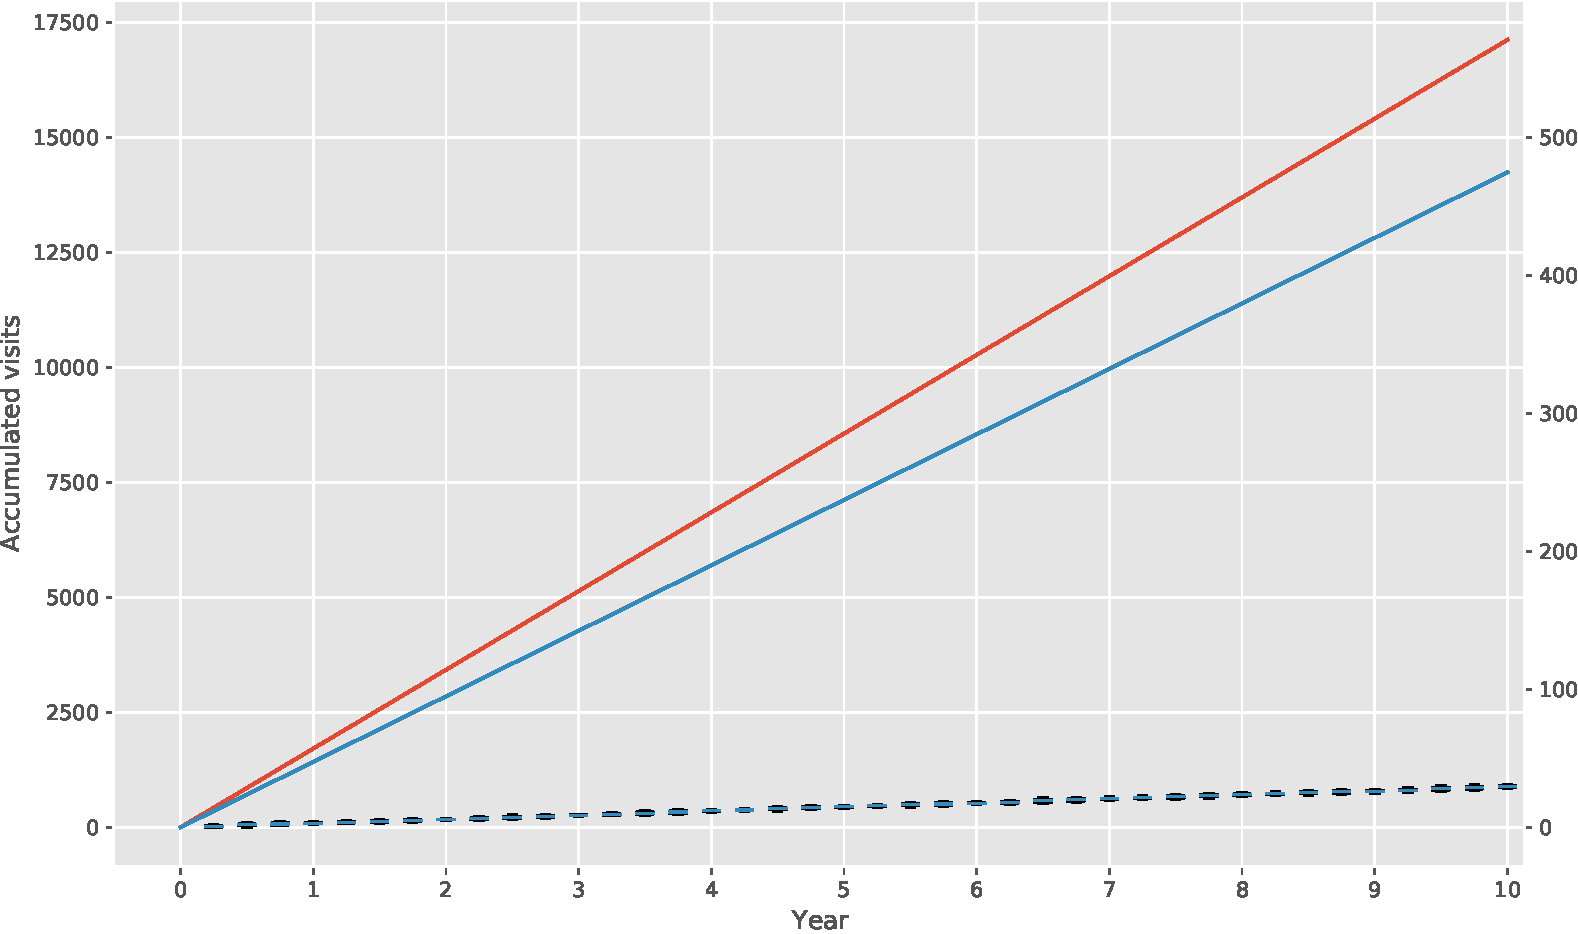
\includegraphics[width=.9\linewidth]{./figures/numvisits_boxplot.pdf}
\caption{\label{fig:orgc82ceb2}Distributions of the number of visits in the best 18000 square degrees by year, for the the 1.7 2 visit baseline. The central line shows the median over the footprint, the box the first and third quartiles, and the whiskers the 5\% and 95\% quantiles. A corresponding figure used for tracking progress should also include indicators of reference distributions, for example by using a shaded background.}
\end{figure}

\begin{figure}[htbp]
\centering
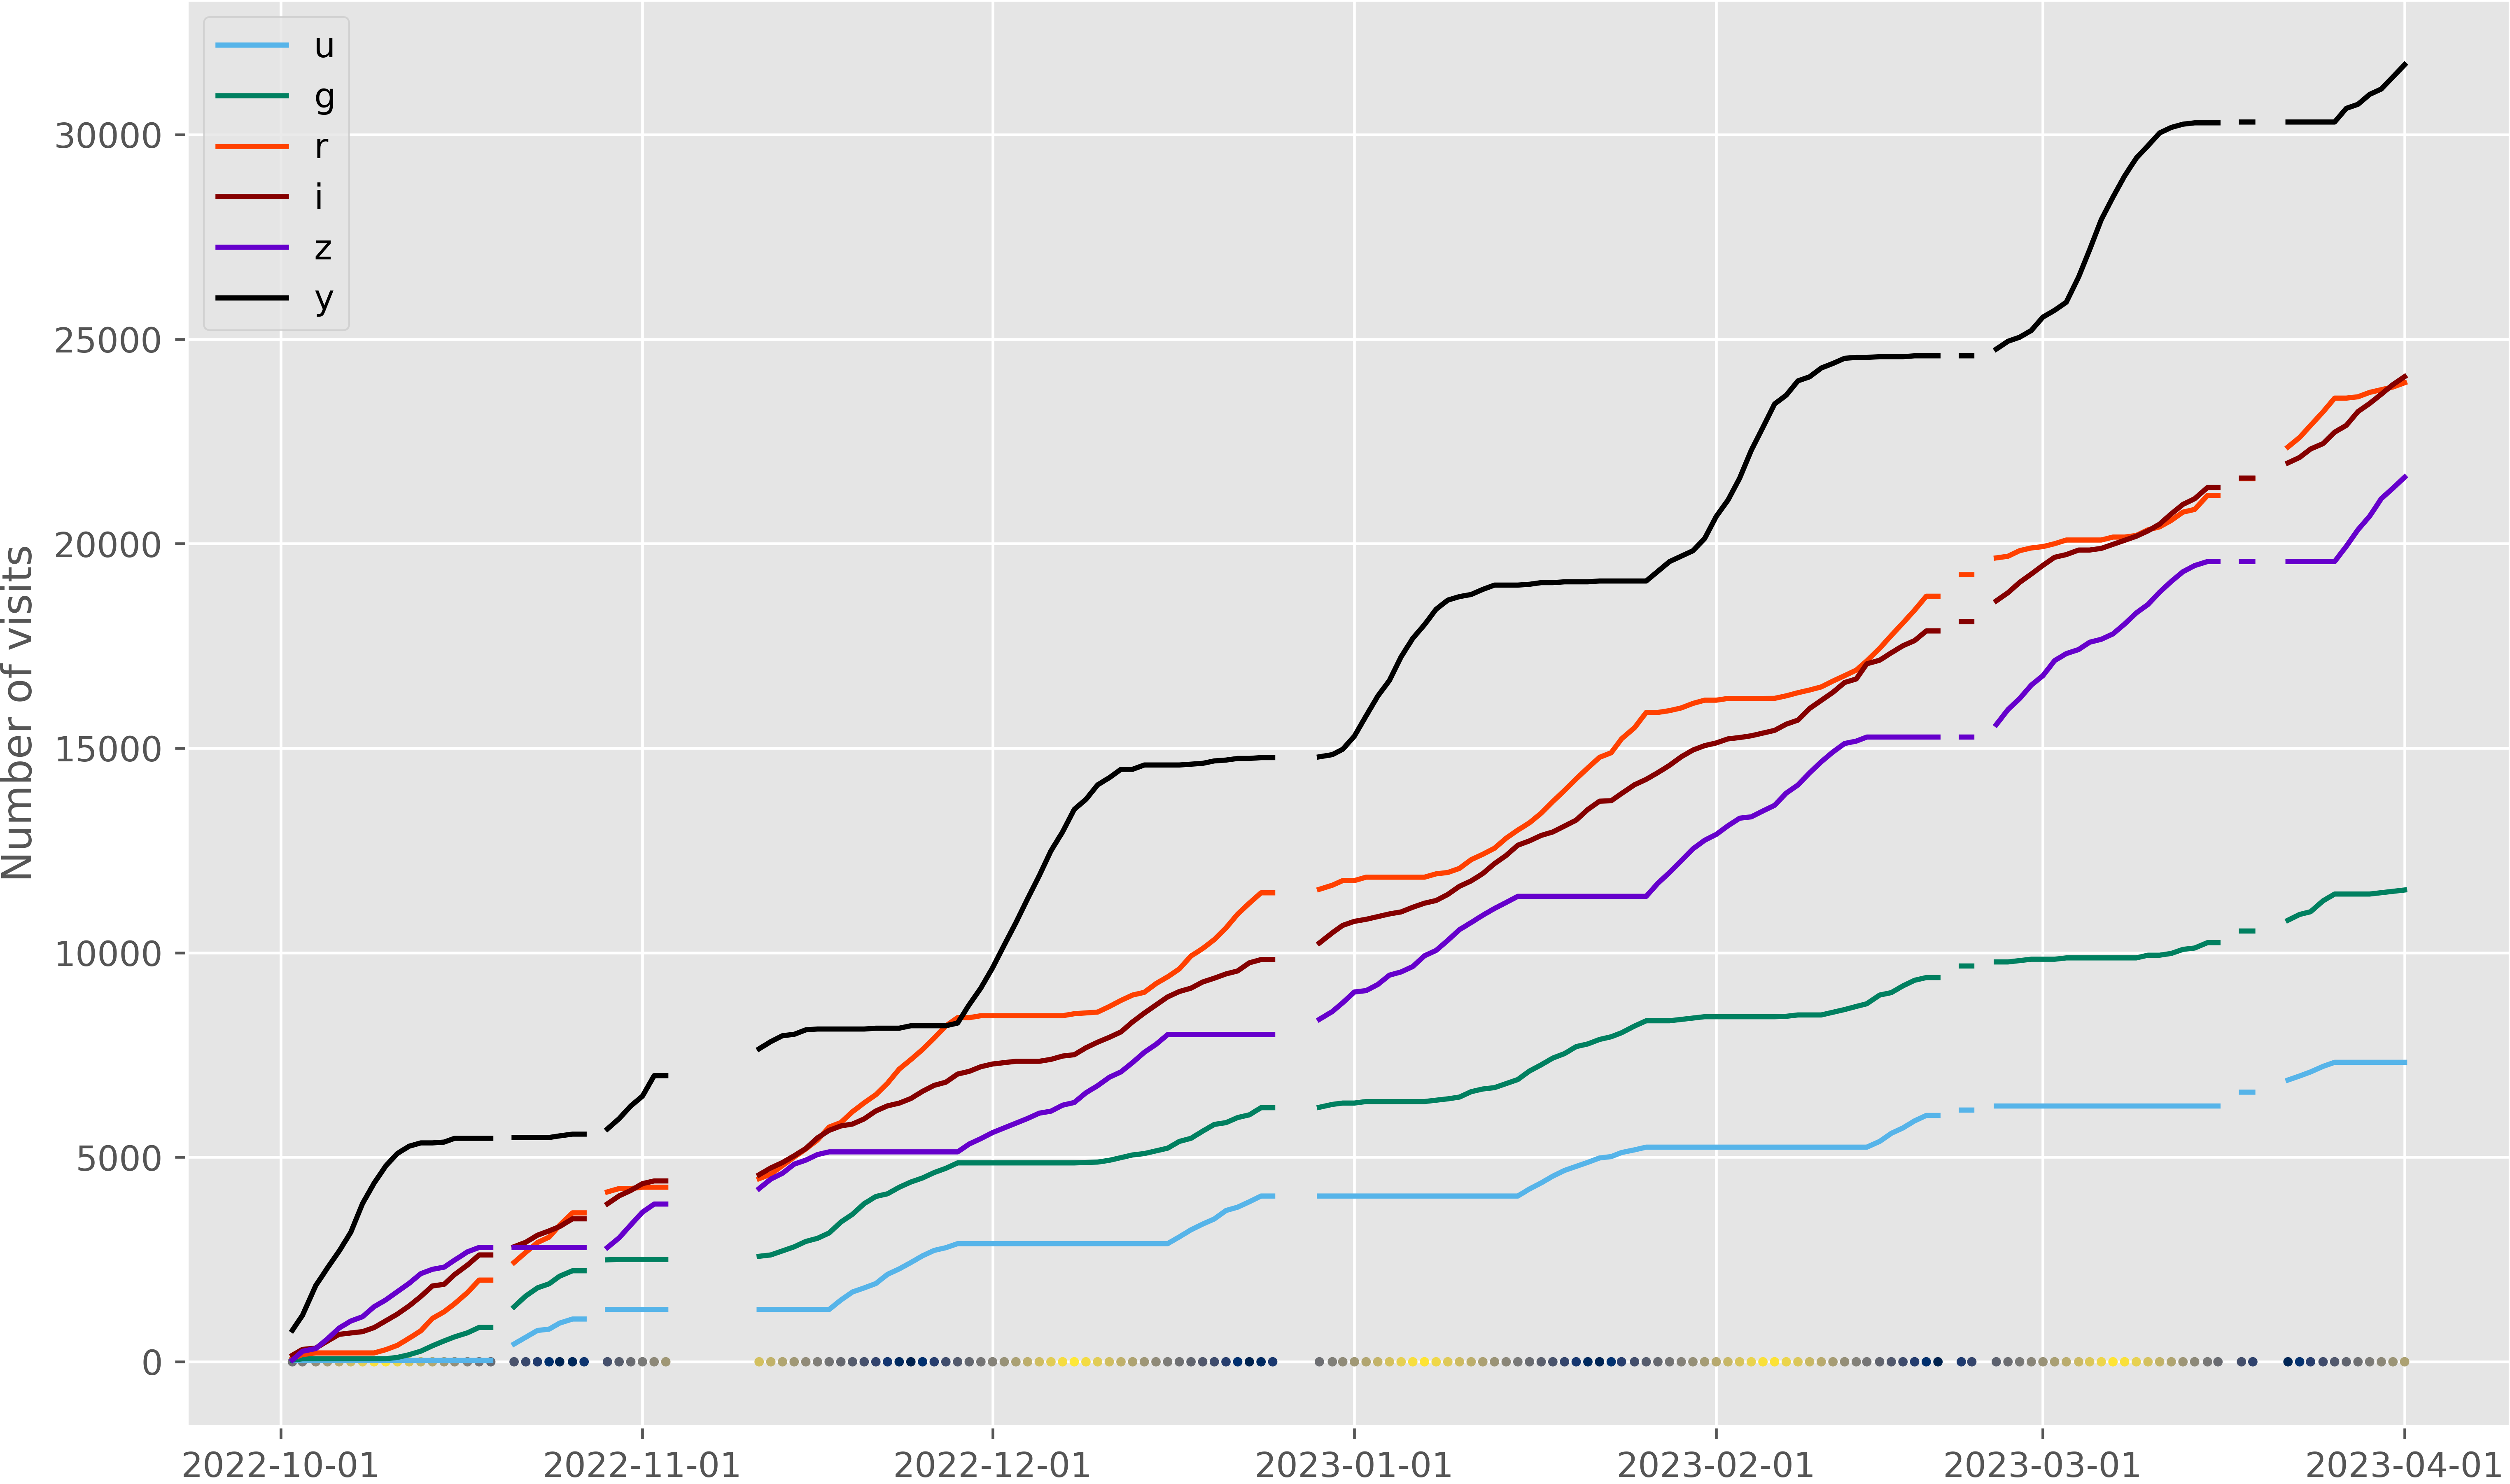
\includegraphics[width=.9\linewidth]{./figures/progress_by_band.png}
\caption{\label{fig:org28f295e}Numbers of visits in each filter as a function of date, with the moon phase along the bottom. A corresponding figure used for tracking purposes should also include indicators of reference distributions, for example by using dashed lines or a shaded background.}
\end{figure}

\begin{figure}[htbp]
\centering
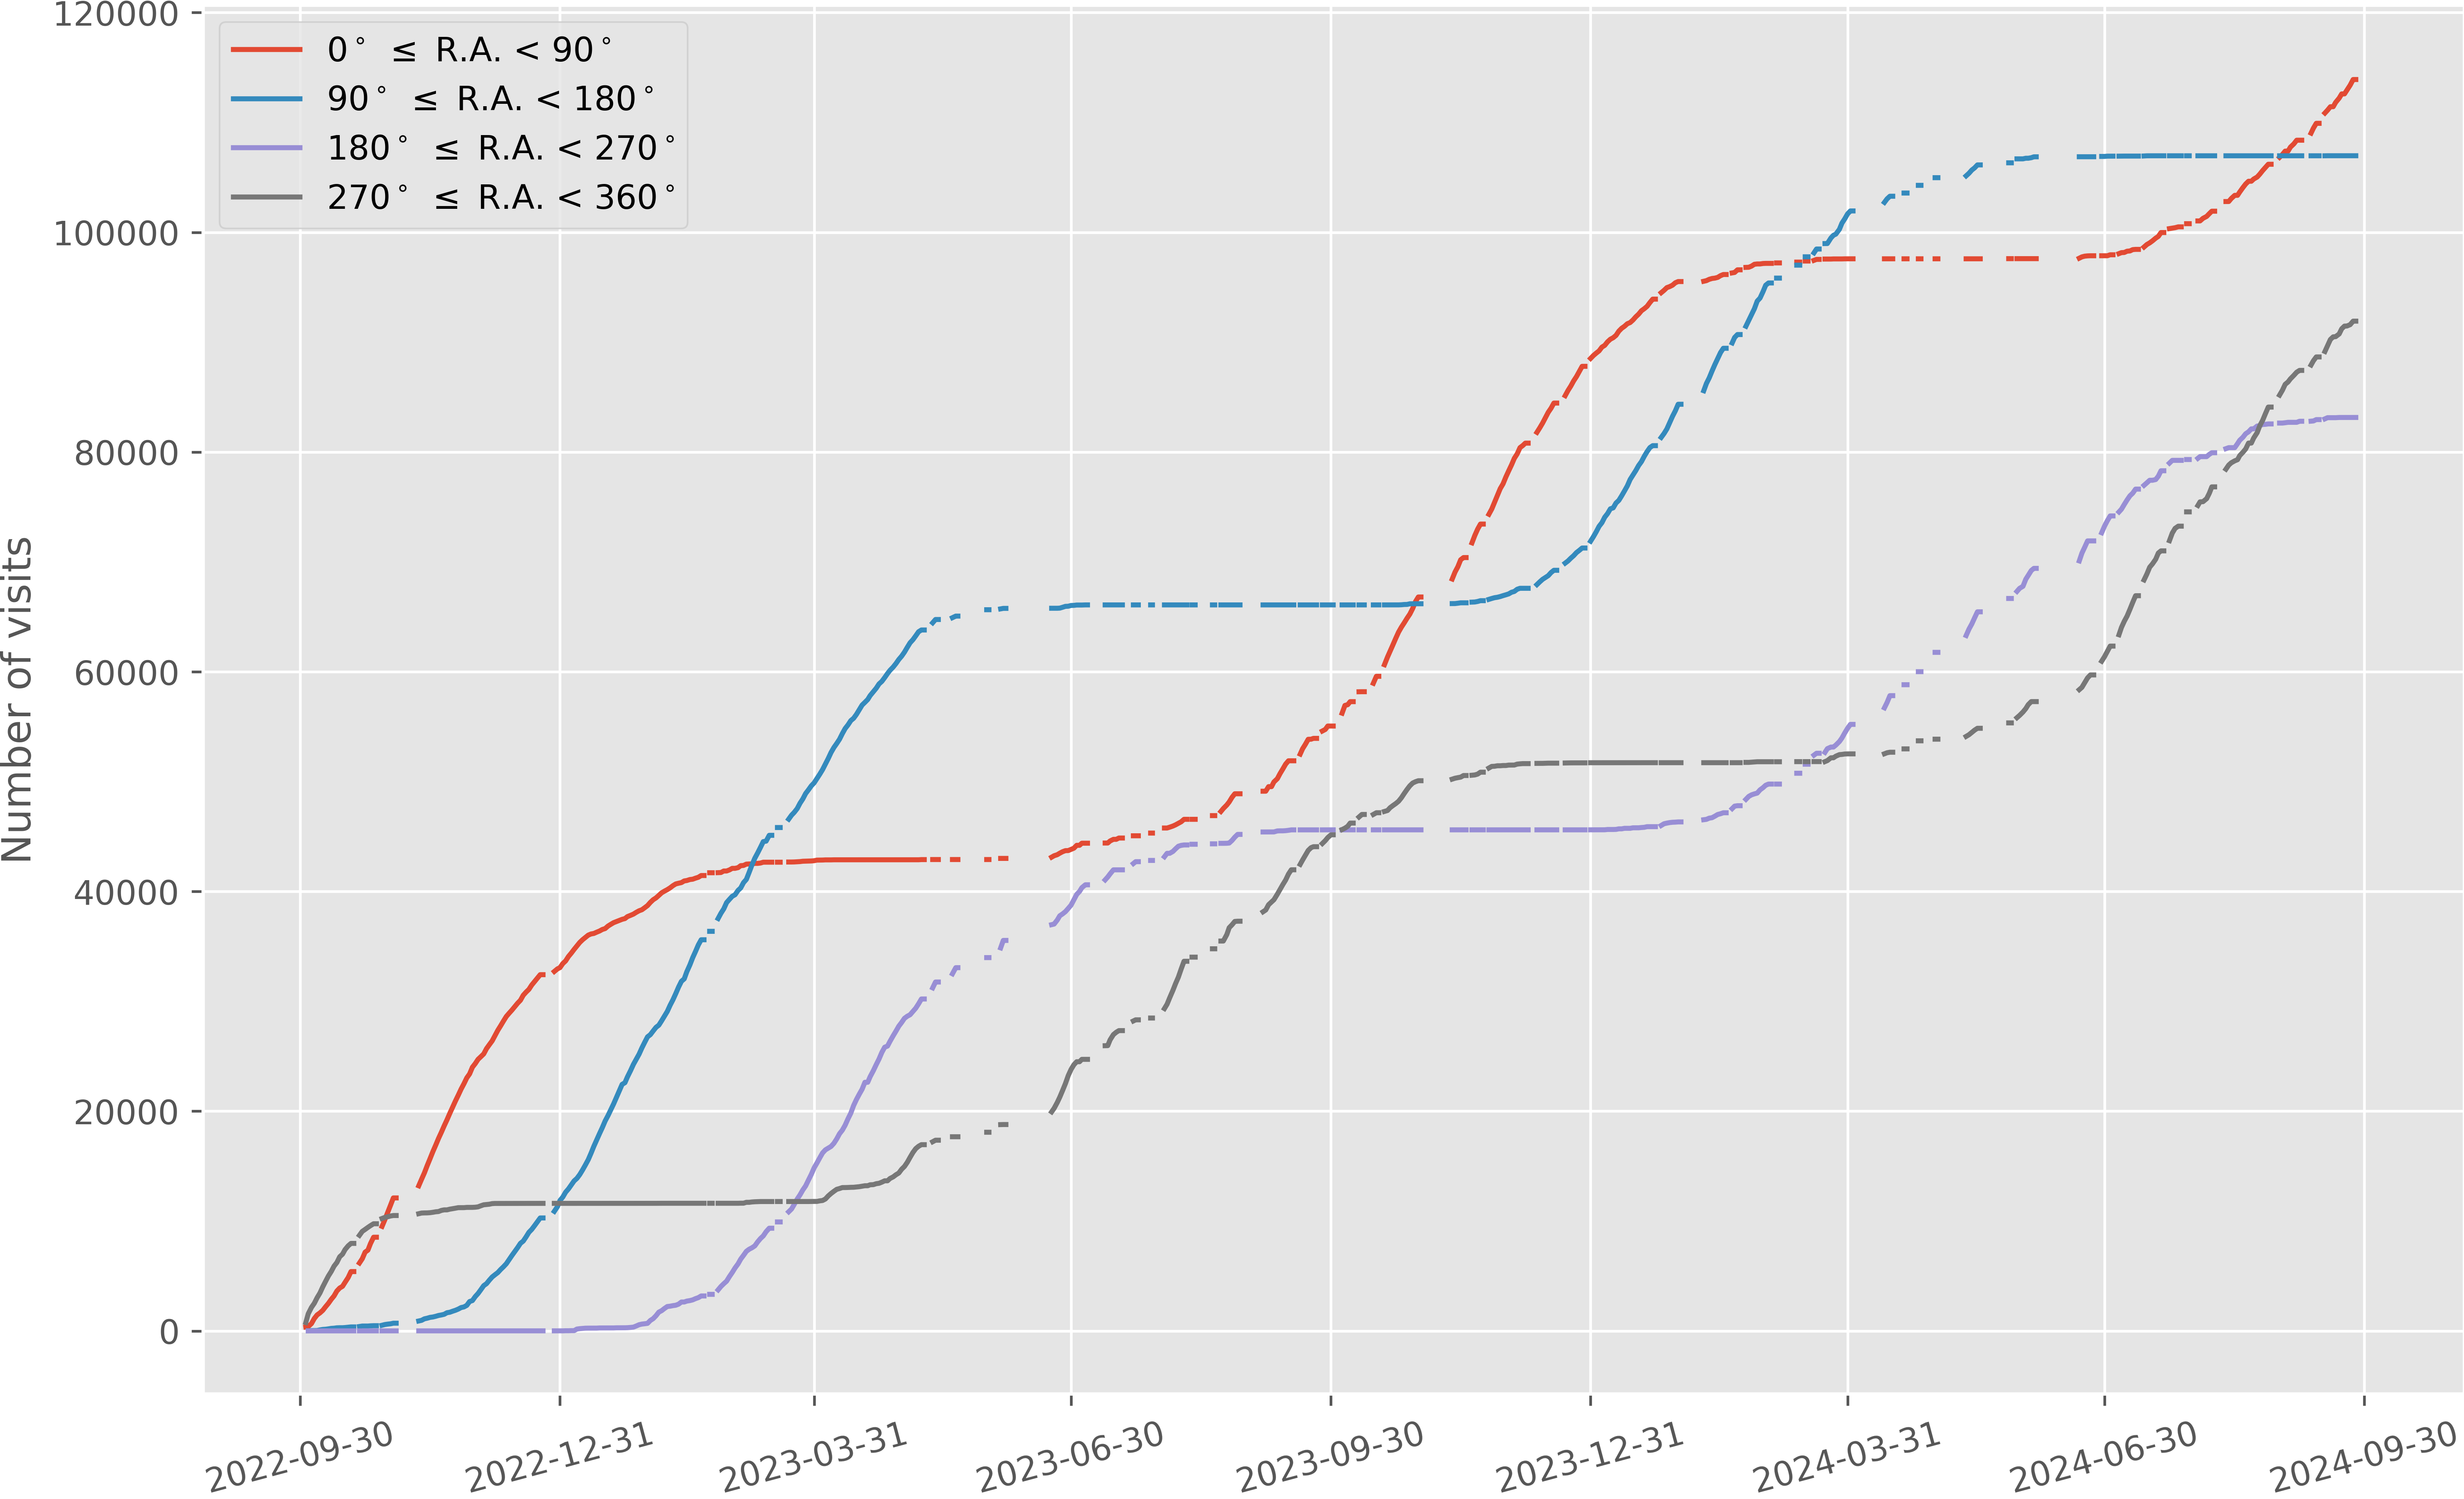
\includegraphics[width=.9\linewidth]{./figures/progress_by_quadrant.png}
\caption{\label{fig:org61d293c}Numbers of visits in each filter as a function of quarter of the sky. A corresponding figure used for tracking purposes should also include indicators of reference distributions, for example by using dashed lines or a shaded background.}
\end{figure}

\subsection{Projected scalar metrics for the final survey as a function of time}
\label{sec:org80a0180}
Many survey metrics do not improve uniformly or even smoothly with time.
For example, the accumulated visits will be spread roughly uniformly over the survey footprint at any given time, so the area of sky observed to the nominal depth (specified in table 22 of \href{http://ls.st/lpm-17}{LPM-17}) will remain near zero for most of the survey, and then rise rapidly at the end: simply tracking the area covered to the nominal depth as a function of time does not provide a useful indication of progress being made toward achieving this metric.
Progress toward achieving this requirement can, however, be tracked using simulations: if the remainder of the survey is simulated after each night of observing and the final metrics measured using the final result, the time series can be plotted to indicate how much progress the survey is making in comparison with what is required.
A flat horizontal line will indicate a survey progressing exactly as expected based on simulations.
A rising line will indicate that the survey is making more progress than expected, while a falling one indicates that the survey is falling behind.

The final area is not the only metric for which these simulations are good tools for indicating progress; all scalar science metrics can be plotted in the same way. Plotting a selection of such metrics can show whether the current conditions or strategy are favoring some science goals over others in unexpected ways.
The list of metrics tracked this way should be the same as that in section \ref{sec:orge255ac4}.

\subsection{Nightly scheduler behavior diagnostics}
\label{sec:org444a433}
A number of plots and metrics will be needed to provide useful diagnostic information that can either help explain or predict the scheduler's behavior, or identify potential problems in it.

These metrics can be usefully tracked at two times:
\begin{description}
\item[{start of night}] At least one \texttt{opsim} simulation should be run for the night before each night of observing. Nightly scheduler behavior diagnostics should be calculated for these simulations, giving an indication of what is expected for the night, and providing advanced warning for any unexpected or anomalous behavior. Nights of observing do not always proceed according to plan: slight differences in the start time or overhead between exposures may cause the predicted and actual schedule to diverge, and closures due to poor weather or equipment failure may create greater disruption. A handful of simulations with random offsets in start times and overheads between exposures can indicate the range of possibilities.\footnote{If the scheduler is modified to respond to observing conditions, then a handful of weather conditions will need to be simulated as well.}
\item[{end of night}] Nightly scheduler diagnostics should be calculated for each night shortly after the completion of observing. These diagnostics will alert the project to any scheduler problems or misbehavior during the night, and help explain the scheduler's behavior when it was not intuitive.
\end{description}

Examples of such diagnostics include:
\begin{description}
\item[{Astronomical maps}] Diagrams resembling planispheres (e.g. shown in figure \ref{fig:orgc07ebd2} are helpful for understanding what parts of the survey footprint are available, which DDF fields might be observed and when, and the degree to which the moon will be a factor in scheduling. Such diagrams do not themselves present progress or scheduler information, but the do provide valuable context in which other scheduler diagnostics should be evaluated.
\item[{Feature maps}] Modern version of \texttt{opsim} select visits (or sets of visits grouped into "blobs") based on "features" that are functions of location on the sky: the slew time to reach the location on the sky, the expected depth of exposures to be taken there, and the progress made so far on that portion of the sky. A weighted mean of these features determines the selection of the next visit or set of visits. Examination of maps of these visits and the resultant final reward function is therefore fundamental to understanding the scheduler's behavior. The presentation of the feature maps is complicated by the variability with time and dependence on current pointing. It may be most useful simply to exclude the slew time feature, which depends on the current pointing. Two candidate formats may be useful for dealing with the time variability:
\begin{description}
\item[{animation}] a movie of the map over the night will provide the most detail, but can be difficult to navigate.
\item[{maximum feature values}] maps of the maximum value each point on the sky takes over the course of the night will be a useful indicator of how likely the scheduler is to schedule visits in these areas at some point in the night.
\end{description}
\item[{Full table of scheduled visits}] To support coordination between Rubin Observatory and other projects, \href{https://ls.st/lse-61}{LST-61}/DMS-REQ-0353 requires that "A service shall be provided to publish to the community the next visit location and the predicted visit schedule provided by the OCS. This service shall consist of both a web page for human inspection and a web API to allow automated tools to respond promptly." Such a table (in both forms) will be useful not only to external projects, but also to the observing scientists: although on most nights the scientist will not need to consult the table, it will sometimes be useful as a reference for exploring the details of expect from the upcoming night when higher level depictions of the night are unexpected or confusing.
\item[{Pointing movie}] A movie of the pointings of the telescope over the course of the night will be one of the fastest ways to convey an understanding of what the scheduler will do (before the night) or did (after it). Superposition of the pointings over the feature map would also help understand scheduler behavior.
\item[{Global observing efficiency}] The ratio of the total science exposure time to the available time (measured using morning and evening twilight as references) provides a good, gross indicator of whether the scheduler is scheduling visits efficiently (minimizing overhead time).
\item[{Gap distribution}] A histogram of the gaps in time between successive visits can indicate where inefficiencies in observing come from.
\item[{Table of long gaps}] Long gaps between exposures indicated either problems or inefficiencies. A short table of unusually long gaps between pairs of exposure with possible indicators of explanations (e.g. the slew angle between exposures, or whether there was a filter change) can call attention to this lost time for evaluation by a human.
\item[{H.A. distribution}] The distribution of hour angles for scheduled exposures indicates whether the scheduler is maximizing data quality.
\item[{DDF cadence plots}] The DDF cadence plots described in section \ref{sec:org3a7f0df} will also be important for understanding whether a DDF should be (or should have been) observed on a given night.
\item[{Fraction of time in blobs}] The "blob" scheduler is intended to be the workhorse scheduler for the WFD, and if an unexpectedly large number of exposures are being scheduled by the greedy scheduler, it may indicate a problem.
\end{description}

\begin{figure}[htbp]
\centering
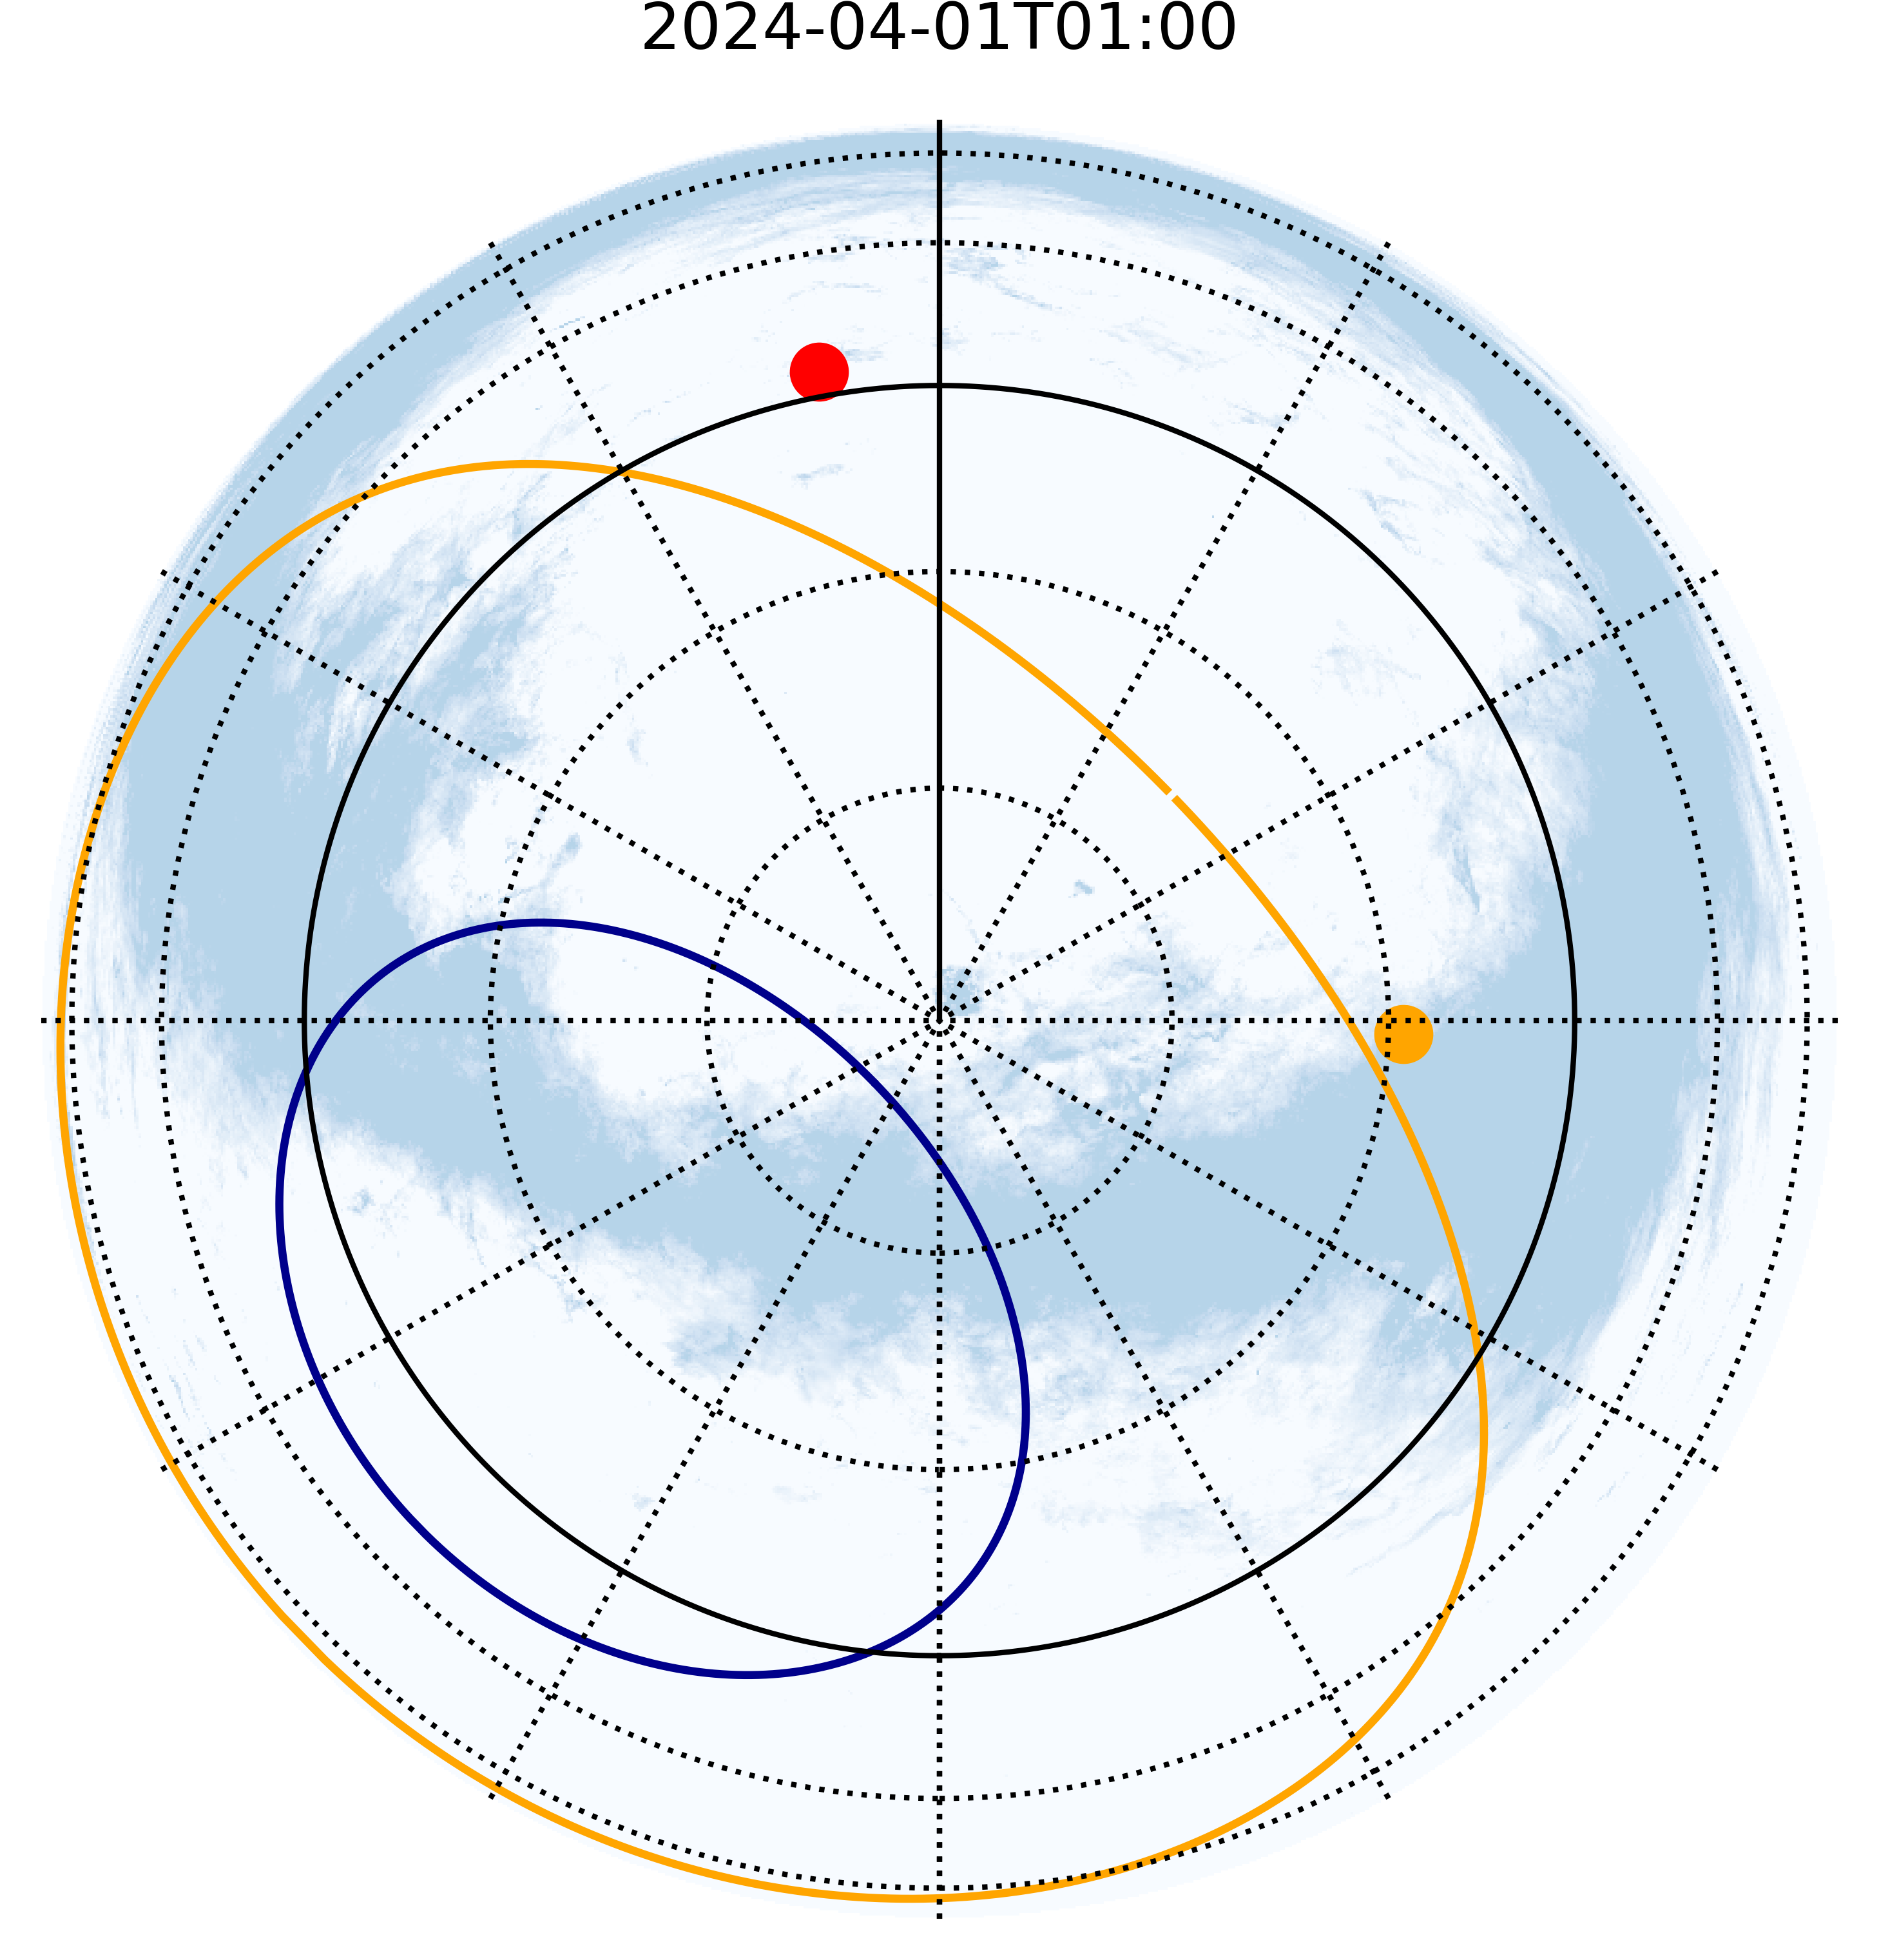
\includegraphics[height=0.4\textheight]{./figures/airmass_map.png}
\caption{\label{fig:orgc07ebd2}An example planisphere diagram, showing the airmass=1.5 altitude circle (blue oval), horizon (orange circle), ecliptic and sun (green circle and star), moon (orange circle), areas of high extinction from dust in the Milky Way (blue shaded area) and brightest stars. Positions of DDF fields boundaries of the WFD survey footprint may also be added.}
\end{figure}

\subsection{Global scheduler behavior diagnostics}
\label{sec:orgdafac3c}
In addition to scheduler diagnostics designed to track scheduler performance on a nightly basis, the project also needs track scheduler behavior for issues that might only become apparent on longer timescales.
An example of this is verifying that the scheduler is observing fields near transit when possible, and that when it observers at pointings far from transit, that there is a well understood reason.
One way of showing this is through an hour angle hourglass diagram, particularly when paired with the time use hourglass plot.
Figure \ref{fig:orgef69f9e} shows an example on such a diagram.
The greatest sustained deviations from observing at transit (an hour angle of \(0^{\circ}\)) occur just before and after the transit of the moon: when the moon is at a low hour angle, the scheduler observes at a high hour angle, and vice versa.
This is reasonable behavior for avoiding brightly moonlit sky.
On shorter timescales, some blocks of exposures at low hour angle are apparent.
Comparing these hourglass plots to the time use hourglass plot (figure \ref{fig:org1a3263e}), it can be seen that these are DDF fields, and that they are being observed well before transit.
The DDF fields, therefore, are being observed at earlier times than optimal in these simulations.

\begin{figure}[htbp]
\centering
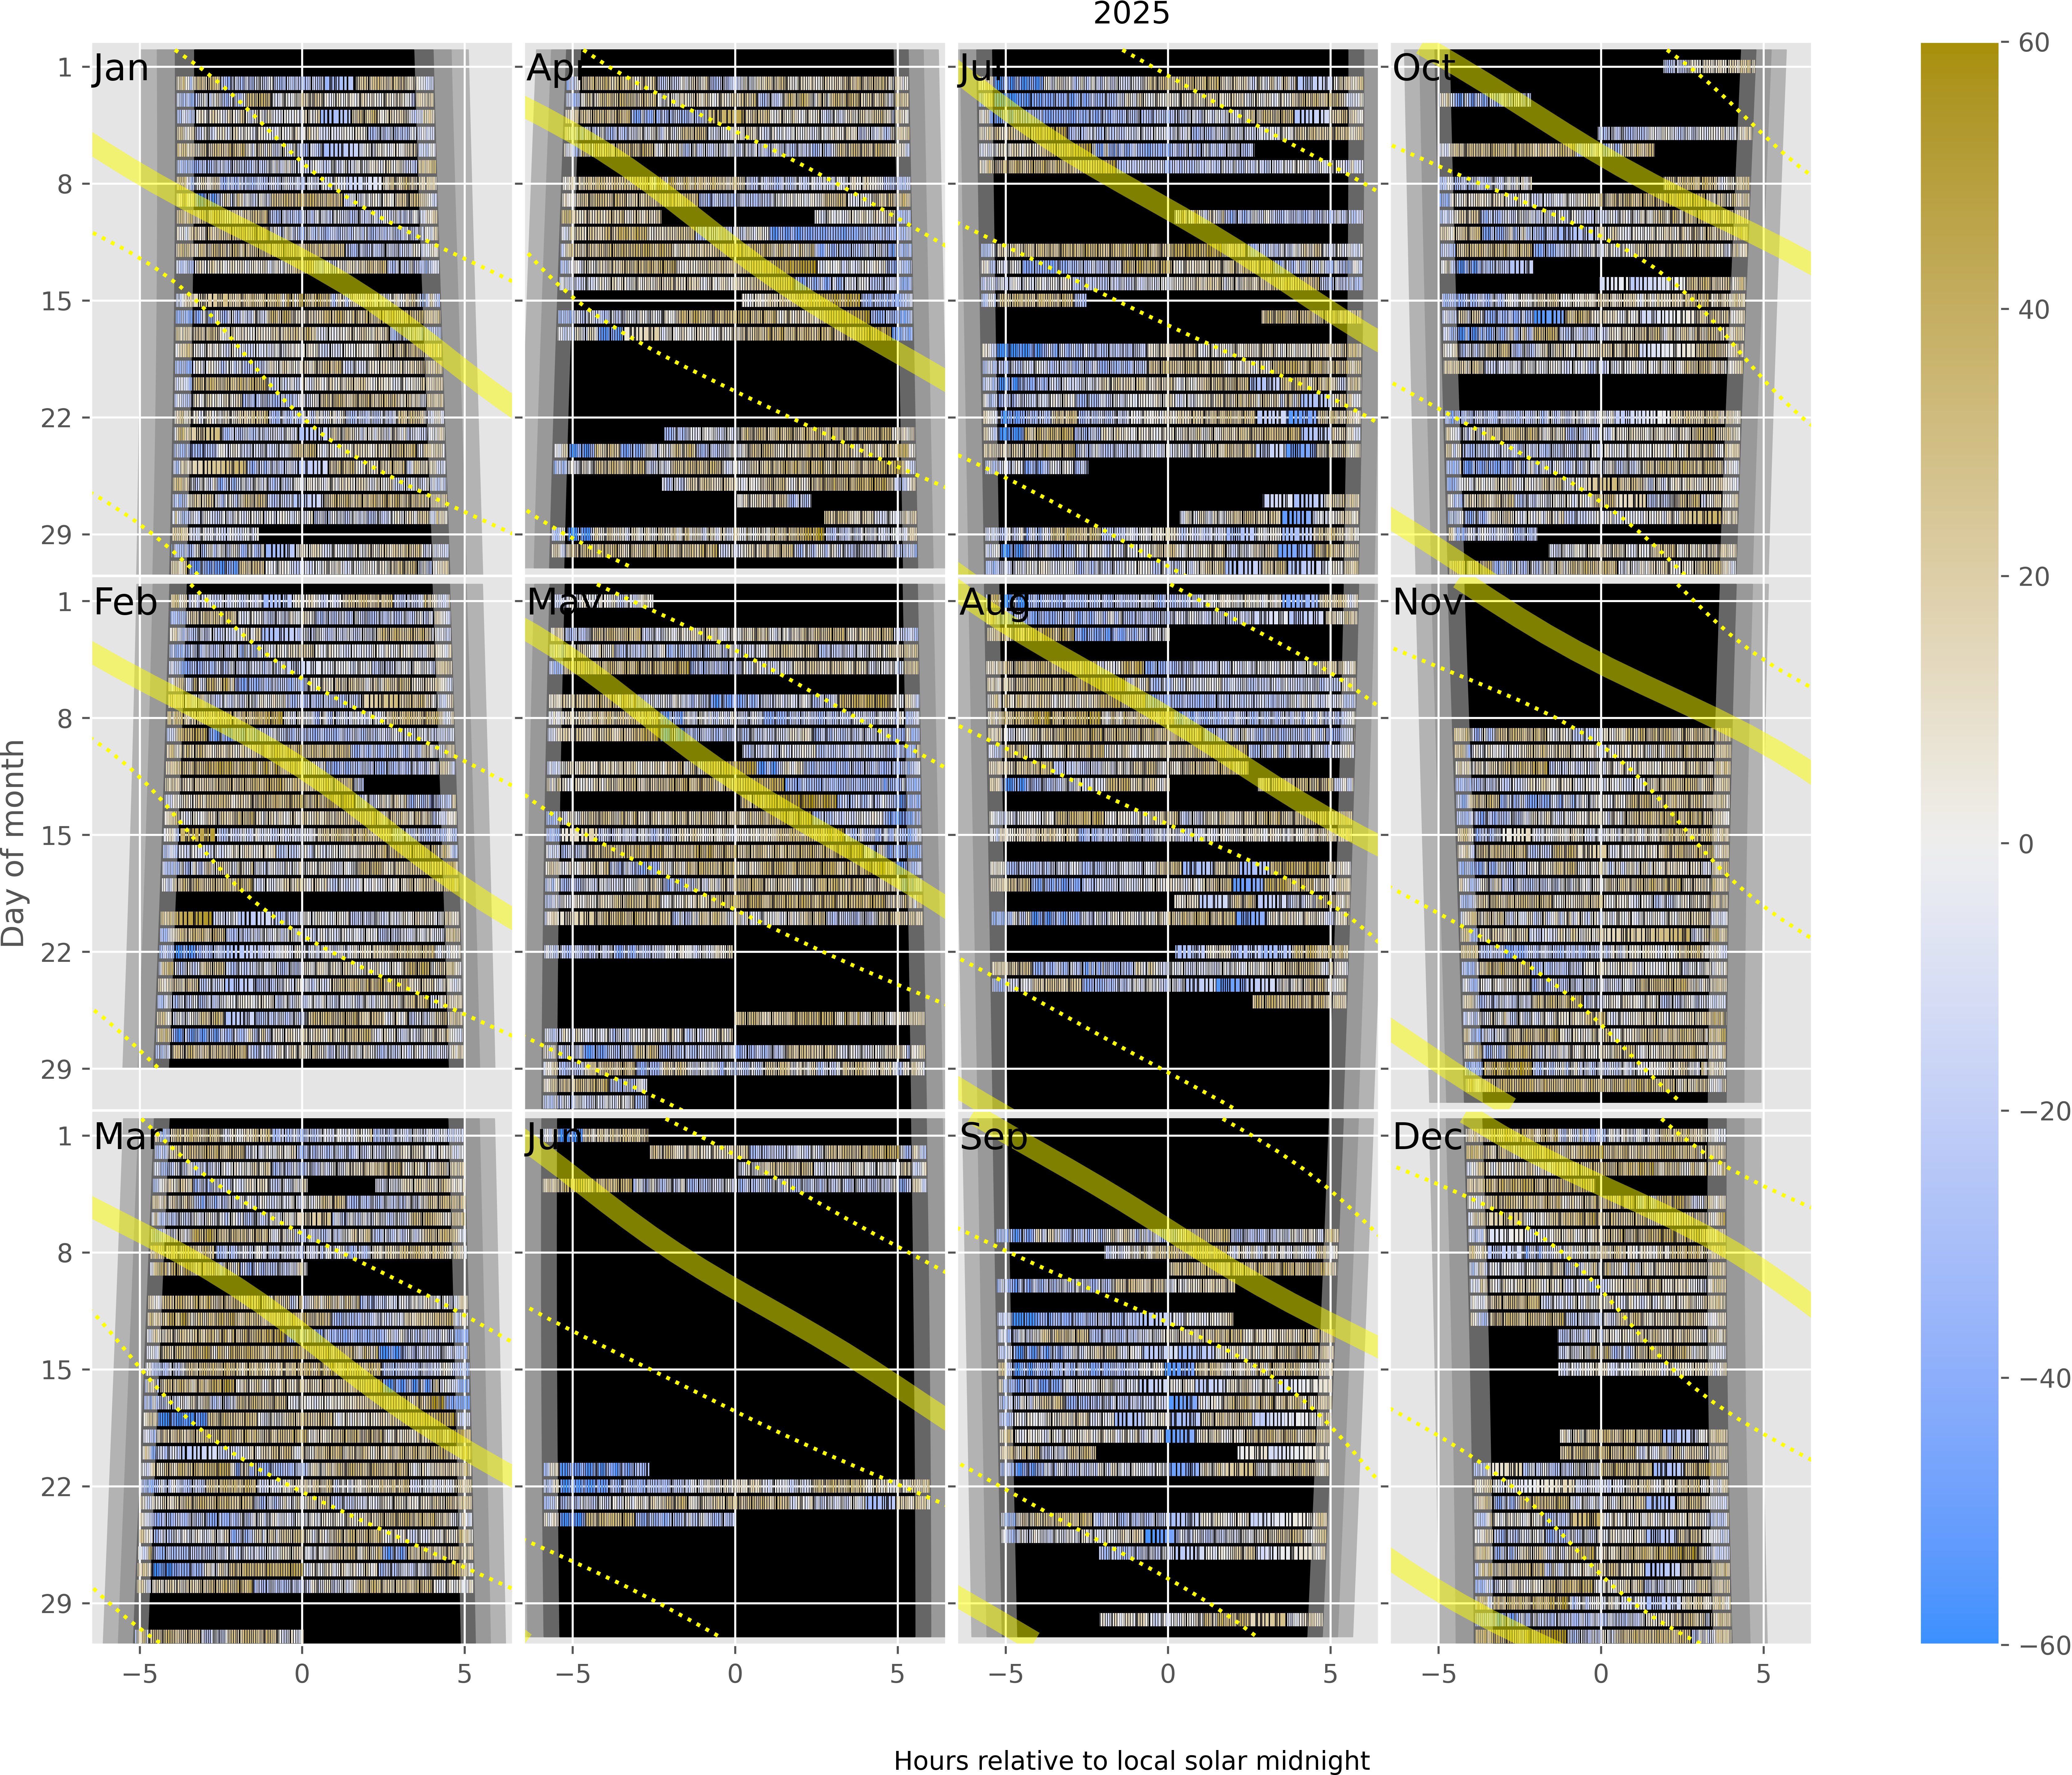
\includegraphics[width=1.0\textwidth]{./figures/hour_angle_hourglass.png}
\caption{\label{fig:orgef69f9e}Example Hour Angle hourglass plot, for one year of the 10 year baseline simulation. The gray and black background shading mark civil, nautical, and astronomical twilight times, and full dark. The thick yellow lines mark the transit of the moon, and the dotted lines, the lunar rise and set times. Colors mark the hour angle of visits taken an the given time.}
\end{figure}


\subsection{Validation of the site and telescope model}
\label{sec:org5c6abb5}
\texttt{opsim} simulations rely on several models for the characteristics of the site and the performance of the instrument.
Deviations from the models can have significant consequences for the accuracy of the simulations.
Comparisons between the modeled and achieved characteristics of the site and instrument will be important not only for understanding deviations between simulated and achieved performance, but also for improving simulations and making corresponding refinements to survey strategy.

For each modeled feature, there are at least two plots are of interest: one plots the measured values against the value calculated by the \texttt{opsim} model; and the other that tracks the distribution of residuals over time (for example a box or violin plot).
In some cases, additional plots may also be important.

Examples of modeled characteristics include:
\begin{description}
\item[{slew time}] In addition to simple comparing the modeled to achieved slew time, residuals between the two can be shown as a function of horizon coordinates and rotator angle.
\item[{filter change time}] Nominally 90 seconds plus up to 30 seconds to put the camera into the necessary position.
\item[{shutter time}] Nominally 1 second of overhead per visit.
\item[{readout time}] Nominally 2 seconds, in parallel with any slew time.
\item[{total overhead between successive exposures}] In principle the total overhead can be calculated by combining each source of overhead, but measurements of the total time from one exposure to the next (the start of one visit to the start time of the next) will be an important diagnostic for discovering if the different values combine as expected, and if there are additional sources of overhead that have not been accounted for.
\item[{sky brightness}] The sky brightness as a function of airmass, sun and moon location and phase, filter, and other factors. Plots that show residuals as a function of horizon coordinates may also be useful for indicating limitations in the model due to light pollution, which is not currently included in the model.
\item[{atmospheric seeing}] \texttt{opsim}'s simulation is based on achieved data from the Gemini South DIMM. A comparison of the Gemini South and Rubin Observatory DIMM measurements will provide a diagnostic for resultant limitations.
\item[{final delivered PSF width}] The final delivered PSF width is a function of the atmospheric seeing, filter, airmass, the turbulence outer scale, dome seeing, and other instrumental contributions. In some cases, the value used by the \texttt{opsim} model is highly uncertain (e.g. the turbulence outer scale). Other contributions (for example the effect of the strength and direction relative to the telescope pointing on the dome seeing) are not currently modeled at all.
\item[{extinction and lost time due to clouds}] The modules used for strategy simulation by \texttt{opsim} are based on historical cloud data recorded by humans at the nearby Cerro Tololo Inter-American Observatory. The correspondence between these estimates and actual time lost is highly uncertain.
\item[{time lost due to engineering activities and equipment failures}] 

\item[{achieved depth}] The expected \(5 \sigma\) limiting magnitude for point source detections in each visit is one of the basic "features" used by the scheduler and is affected by a variety of factors. Comparisons between estimated and achieved depth are therefore of fundamental importance.
\end{description}

While some of these characteristics are functions of others, independent measurement of each will be important for verifying that the relations are those that are expected, and that there are no significant unaccounted for contributions.

Often, these characteristics will be tracked as part of telescope operations, independent of direct strategy considerations.
However, tracking and maintaining survey strategy requires presentation in a way that supports easy comparison to and updating of the \texttt{opsim} models.
Either the tracking and monitoring being done for other systems should include the necessary comparisons to the \texttt{opsim} models, or separate variations should be generated for the Scheduling Scientists and Survey Software Engineers.

\subsection{Disruption consequence analysis}
\label{sec:org386f57a}
The project will need to be able to quantify the consequences of departures from the baseline strategy, both in advance and in retrospect. 
Possible causes of disruptions include "target of opportunity" observing, unexpected engineering downtime, and observing in a degraded state (e.g. with a broken raft). 
It some cases, the ultimate consequences for the science will not always be immediately obvious.
For example, a set of target of opportunity exposures will not necessarily result in complete loss of time for the WFD or other programs, because exposures scheduled for the ToO will often contribute to the FWD themselves. 
To quantify the effects of such disruptions, achieved metrics need to be compared to what they would have been without the disruptions.
This comparison requires additional simulations.
By comparing metrics derived from simulations in which the description never takes place with ones in which they did, both the immediate and long-term effects of the disruption can be quantified.
The details of what simulations are needed for the comparison depend on whether the disruption being analyzed is one that has already occurred, or one which is under consideration or expected.
When evaluating possible future disruptions, the simulations for comparison are both simulations from the current time to the completion of the survey, differing only by whether the disruption occurs.
When evaluating the effects of a past disruption, the reference simulation (the one without the disruption) must begin in the past, before the disruption, and be run with the same environmental parameters (e.g. clouds and seeing) as actually achieved.
That way, the consequences of the disruption itself can be evaluated independently of deviations between the simulated and actual survey.

In both cases, short and long-term differences are of interest.
Two disruptions may have similar short-term effects on metrics, but some disruptions will be easier for the automatic scheduler to automatically recover from with future observations than others.
The time and degree to which it will be possible to recover from the disruption will sometimes be important information.

\section{Tools, reports, and their users}
\label{sec:orgcd26199}
\subsection{Introduction}
\label{sec:org6039a05}
The Rubin Observatory project and staff performing LSST will require survey progress and status diagnostics, including a variety of metrics and plots.
Some of these will be needed by the staff themselves, providing the data needed to prevent and diagnose problems, identify potential improvements, and evaluate suggestions for changes.
In addition, such plots and metrics will also be needed for reports to the astronomical community and funding agencies, and even may be useful in engaging the general public.

The infrastructure suitable for producing such plots and metrics depend on several factors, including the audience expected to make use of them and the frequency with which they need to be produced.
Full automation of the production of plots and metrics will be most important when they need to be produced frequently, on a nightly or monthly basis.
When their audience includes non-experts, either full automation or simple production on demand will save effort.
Plots that are used primarily for debugging or exploration of specific issues may not require the same level of automation or simplicity of interface, but tools for reproduction of previous example of such diagnostics can be important for avoiding duplication of effort.

These plots and metrics can be produced and presented in any of several ways:

\begin{description}
\item[{Interactive tools}] When developing and debugging the software, hardware, and human procedures that produce the survey, experts working on the project require flexible tools to obtain and explore the relevant data. Planning and prediction of the consequences of events and choices will often benefit creation of simulations. Examples of such sets of tools (e.g. \texttt{opsim} and \texttt{MAF}) have been developed as part of project construction, and will continue to perform an important role in operations. General tools designed for monitoring other aspects of the survey (e.g. the health of the instrument or the status of data processing) will also have important roles to play.
\item[{Information dashboards}] Some plots and metrics will routine production and monitoring, often by those who are not expert users of the interactive tools like \texttt{MAF}. Even for those who do have the expertise, automation of the production of routine plots and metrics will save significant effort. Infrastructure that generates needed plots and metrics and presents them in a simple way (e.g. an automatically update web page, or small collection of web pages) will therefore be important. This infrastructure will require many of the same software components used by the interactive tools, plus some automation and presentation elements.
\item[{Reports}] The project will need to produce reports covering survey status and progress, whether in the form of documents and presentations. Many of the plots and metrics displayed in an information dashboard will be important elements in these reports.
\end{description}

The intended audience and the frequency of reporting are both important feature to consider in determining how any given metric or plot is to be generated.
Possible audiences include the funding agencies, Rubin Observatory management, LSST science collaboration scientists, the Observatory Science team (including the Observatory Scientist), the Observing Specialists, the Observatory Support Scientists, the Scheduler Scientists, Survey Software Engineers, astronomers working on other projects, other members of the astronomical community, and the general public. 
Plots and metrics may be generated on regular schedules (nightly, monthly, or quarterly), or as occasions demand.

The LSST system and data management requirements (\href{https://ls.st/lse-29}{LSE-29} and \href{https://ls.st/lse-61}{LSE-61}) and observatory systems specifications (\href{https://ls.st/lse-30}{LSE-30}) include requirements on several reports and reporting tools. The roles and activities in the \href{https://docushare.lsst.org/docushare/dsweb/Get/Document-36797/Rubin\%20Observatory\%20Operations\%20Plan\%20April\%202020.pdf}{Rubin Observatory Operations Plan} imply additional reports, and imply additional requirements on those already described.

\subsection{Night Plan}
\label{sec:orgd5471e6}

Potential problems related to strategy or scheduling should be found and resolved before each night of observing, of possible, and the observing specialists on shift during the night need to be briefed and provided with a written plan describing any unusual activities or modes of operation, what they should expect of the scheduler, what behavior they should consider anomalous, and how they should react to anomalous behavior.
The \href{https://docushare.lsst.org/docushare/dsweb/Get/Document-36797/Rubin\%20Observatory\%20Operations\%20Plan\%20April\%202020.pdf}{Rubin Observatory Operations Plan} gives responsibility for reviewing and supervising scheduler behavior to the Observatory Scientist and the Observatory Support Scientists, but specific procedures for this review and the briefing of the observing specialists are not yet developed.
Under any plan, it will be worthwhile to automate the generation of the necessary scheduler simulations and diagnostics (listed in section \ref{sec:org444a433}) for review and inclusion in briefing for the observing specialists and a plan for the night.

In operations rehearsals (summarized in \href{https://dmtn-119.lsst.io}{DMTN-119} and \href{https://dmtn-159.lsst.io/}{DMTN-159}), each night was planned in a daily meeting which included the current status and plans for the next night.
Among the "lessons learned" described in DMTN-119 was the need for a good note-taking during the daily meeting, with status report elements filled in before the meeting itself. 
The minutes of this meeting can then become a plan for the night.
Infrastructure to automate the creation of these report elements could either present them using a dashboard-like interface and be incorporated into the minutes, or create a template night plan directly, then supplemented during the meeting.\footnote{This process is similar to that used for observing for the Dark Energy Survey (DES).}

Automation in support of the night plan should include:
\begin{itemize}
\item Automatic creation of one or more scheduler simulations.\footnote{A side effect of the creation of scheduler simulations completed in the afternoon is the creation of one or more candidate schedules. If these are produced in format that can be uploaded to the OCS, they can serve as a back-up to the scheduler in the unlikely event of a catastrophic failure of the scheduler during the night.}
\item Automatic creation of the diagnostics listed in section \ref{sec:org444a433}, based on the simulations.
\item Presentation of the diagnostics a dashboard, automatically generated static report, or as part of a template observing plan for the night.
\end{itemize}

\subsection{Published upcoming schedule}
\label{sec:org84e90d3}
To support coordination between LSST observing and that of other projects, including scheduling of simultaneous or nearly simultaneous exposures the same areas of sky, the requirements specify that Rubin Observatory publish the observing schedule in advance.

One requirement that specifies the advanced schedule is \href{https://ls.st/lse-61}{LST-61}/DMS-REQ-0353, "Publishing predicted visit schedule":
\begin{quote}
Specification: A service shall be provided to publish to the community the next visit location and the predicted visit schedule provided by the OCS. This service shall consist of both a web page for human inspection and a web API to allow automated tools to respond promptly.

Discussion: The next visit and advanced schedule do not need to be published using the same service or protocol.
\end{quote}
another is \href{https://ls.st/lse-30}{LSE-30}/OSS-REQ-0378, "Advanced Publishing of Scheduler Sequence":
\begin{quote}
The scheduling of the observing sequence lasting at least \texttt{schedSeqDuration} shall be published in advance of each observing visit.
\end{quote}

These requirements imply the infrastructure necessary for:
\begin{itemize}
\item Automatic creation of scheduler simulations. The initial simulation for the night may be the same one as that described in section \ref{sec:orgd5471e6}, but additional simulations throughout the night will also be required.
\item A service to publish the predicted schedule through a web API.
\item A service to publish the predicted schedule on a web page suitable for human inspection.
\end{itemize}

The overlap between these requirements and those for the creation of a night plan suggests that the same tool be used for both uses. 
Support for this use case imposes several additional requirements not present for the night plan:
\begin{itemize}
\item The published schedule and diagnostics must be available to the public, not just the project staff.
\item Update schedules need to be published as necessary through the night, not just at the start of each night.
\item A web API suitable for support of automated tools must be supplied.
\end{itemize}

\subsection{Night reports}
\label{sec:orgfa64fd4}
Night reports (or nights summaries) are in important feature common to most astronomical facilities, and basic plots and metrics indicating survey progress are important elements for such reports in large surveys such as LSST.
Several Rubin Observatory requirements require specify different aspects of the content and creation of night reports, including LSE-30/OSS-REQ-0131, LSE-30/OSS-REQ-0406, LSE-61/DMS-REQ-0096, and LSE-61/DMS-REQ-0097. Section 1.4 of LST-490, the "Observatory Electronics Logging Working Group Report," acknowledges the need for infrastructure to support the creation of this report.
The specifications require that the report summarize "per system performance and behavior," but do not specify what is to be reported in great detail.
This report is a natural home for the nightly scheduler behavior diagnostics (described in section \ref{sec:org444a433}), when applied to actual (as opposed to simulated) scheduled nights.
Furthermore, some elements of the survey state description (section \ref{sec:org3a7f0df}) will be of broad enough interest that updates to them may be usefully included after each night.

In addition to the diagnostics directly related to scheduling, several of the data quality indicators that will be reported in the night report (following LSE-61/DMS-REQ-0097) to monitor the health of other subsystems are close to those needed for validation of the scheduler's site and telescope model (section \ref{sec:org5c6abb5}). If these elements are produced with the needs of the scheduler scientists in mind, these same plots may fill both needs.

So, to support scheduler and survey progress monitoring, the night report should include:
\begin{itemize}
\item Comparisons of system characteristics (slew time, filter change time, depth, sky brightness, etc.) with models used by the scheduler simulator (some subset of the diagnostics listed in section \ref{sec:org5c6abb5}).
\item Nightly scheduler behavior diagnostics (most or all diagnostics listed in section \ref{sec:org444a433}).
\item Updated diagnostics for the survey state (a selection of the diagnostics listed in section \ref{sec:org3a7f0df}).
\end{itemize}

\subsection{Tools for performance evaluation and analysis}
\label{sec:orgcdb7e30}
The Observatory Scientist, Observatory Support Scientists, and the Survey Scheduling team will need to routinely monitor survey progress and assumptions at a more detailed level than supported by the night reports alone:
detailed monitoring will require all diagnostics listed in section \ref{sec:org922c37a}.
Furthermore, additional diagnostics will be required to debug specific problems, understand anomalies, and evaluate changing conditions or survey priorities.

In most cases, the different diagnostics will depend on a common set of data, including:
\begin{itemize}
\item observatory telemetry
\item one or more baseline survey simulations
\item the record of the visits completed up to and including the most recent night (including data quality information)
\item simulations of the future of the survey, starting with the next night of observing.
\item previously completed survey simulations, starting after each completed night of observing.
\end{itemize}

In some cases, analysis for scheduling and survey strategy may use tools developed for other purposes, such as maintenance of the instrument itself (as specified in \href{https://ls.st/lse-30}{LSE-30}/OSS-REQ-0067).
In other cases, analysis will require more flexible computation or access to data, including creation of custom scheduler simulations, access to archives of completed scheduler simulations, data management results, or even external data sources.
Once code for creation of a diagnostic is developed, the processes and tools used should support easy or automatic regeneration of the diagnostic.
When the creation is not computationally expensive, including it in a set of diagnostics to be automatically regenerated and posted nightly should be straightforward.
For computationally expensive diagnostics, inclusion in a set of diagnostics that can be repeated "on demand" should be similarly straightforward.

The set of tools available to the Survey Scientist, Survey Support Scientist, and the Survey Scheduling team should therefore include:
\begin{itemize}
\item APIs that provide access to observatory telemetry, archives of survey simulations, and DM output from within a common environment. These tools will therefore require access to either the summit Engineering and Facilities Database (EFD, \href{https://ls.st/sql-034}{SQR-034}) or the data management EFD (DM-EFD, \href{https://ls.st/sqr-029}{SQR-029}) for the telemetry data, and the DM butler for access to DM output. Access to an archive of past \texttt{opsim} simulations and the metrics calculated from them will also be required. That can be achieved by any of several means, including a simple filesystem.
\item A computational environment that includes the analysis and tools needed for computing diagnostics (e.g. jupyter notebooks with environments that include \texttt{opsim}, \texttt{MAF}, and standard python scientific libraries)
\item Tools for automatic execution of lightweight code written to calculate diagnostics.
\item Tools for on-demand execution of computationally expensive diagnostic calculation.
\item A tool for collection and presentation of calculated diagnostics.
\end{itemize}

\subsection{Periodic progress reports and performance reviews}
\label{sec:org8a6fc26}
The observatory staff and scheduling team will need to report progress and strategic concerns to management, funding agencies, and the community as a whole. Requirements for the existence of such reports are present in multiple plans and requirements documents. Some examples include \href{https://ls.st/lse-29}{LSE-29}/LSR-REQ-0065, "Survey performance reviews," which states:
\begin{quote}
The Observatory shall have the ability to provide periodic status reports on the progress of the survey to allow both operations staff and the community to assess the survey progress.
\end{quote}
and \href{https://ls.st/lse-30}{LSE-30}/OSS-REQ-0033, "Survey Planning and performance monitoring", calls out the need for reporting to the community at large:
\begin{quote}
The LSST shall provide the tools and administrative processes necessary to monitor the progress of the ongoing survey, provide reports on the progress of the survey, respond to feedback from the science community, and evaluate the impact of changing science priorities over the 10 year survey lifetime.

Discussion: It is expected that the performance of this task will require the use of detailed survey simulations to evaluate scheduling alternatives and optimize the future performance of the survey.
\end{quote}

The \href{https://docushare.lsst.org/docushare/dsweb/Get/Document-36797/Rubin\%20Observatory\%20Operations\%20Plan\%20April\%202020.pdf}{Rubin Observatory Operations Plan} gives responsibility for producing a quarterly report to the Observatory Support Scientist:
\begin{quote}
Responsible for producing a quarterly report on the scheduled/expected observations versus the performed observations. This analysis includes monitoring the assumptions used by the scheduler including slew times, shutter open/close times, readout times etc. 
\end{quote}

Multiple reports will be made on different schedules, customized for different audiences.
All of these reports may draw from any of the report elements described in section \ref{sec:org922c37a}, but it is unlikely that any single report will require every element.
While the generation of individual elements will benefit from automation, the compilation and construction of such reports will require human attention and customization to each audience.

\subsection{Interfaces for education and public outreach}
\label{sec:org67432c6}
While many survey progress metrics and visualizations are only likely to be of interest to experts, several will be intuitive, and may be good candidates for engaging the general public, as per \href{https://ls.st/lse-29}{LSE-29}/LSR-REQ-0113, "EPO Products, Tools, and Interfaces"
\begin{quote}
LSST EPO shall provide access to LSST data through tools, interfaces,
and learning experiences that are designed to engage communities with
different levels of knowledge, experience and skills.
\end{quote}
Good candidates for presentation to the public are movies of numbers of exposures generated, and plots numbers of galaxies (or other objects) detected as a function of time.
\section{Workflows and infrastructure}
\label{sec:org970d5fc}
\begin{figure}[htbp]
\centering
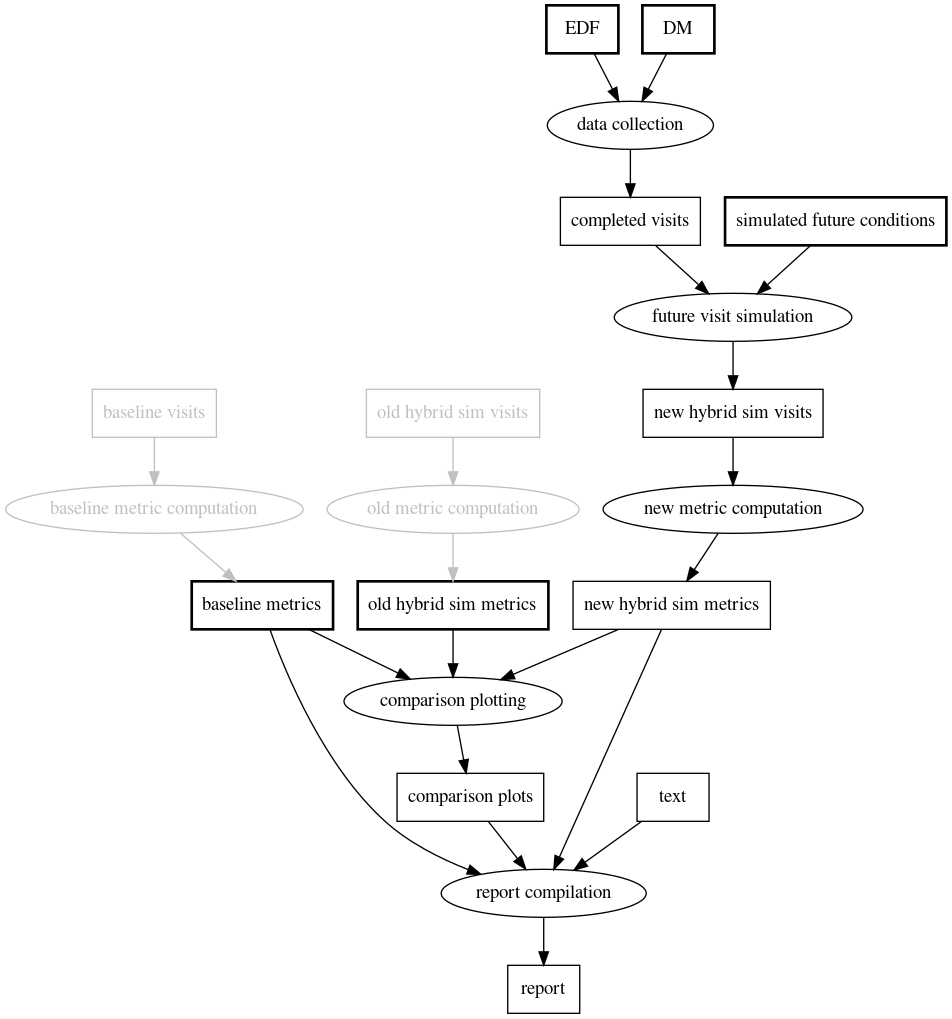
\includegraphics[height=0.9\textheight]{./figures/reportdfd.png}
\caption{\label{fig:org5f7d690}A data flow diagram for producing an LSST observing progress report. Lighter gray elements represent those that need not be repeated every night. Heavier boxes indicate input to the workflow.}
\end{figure}

The workflow for producing reports will have several steps, each reading some sets of data, and producting others. Figure\textasciitilde{}\ref{fig:org5f7d690} shows the data flow for the production of a progress report:

\begin{description}
\item[{data collection}] Progress reports require databases of visits, including observing parameters and basic metadata on each visit. Examples of such metadata will include the depth and sky brightness. This process collects the required data from the Engineering and Facilities Database (EFD) and the output of data management (probably from an instance of a DM butler) and produces a visits table, probably similar to the sqlite databases currently produced by \texttt{opsim}.
\item[{future visit simulation}] In general, it will not be sufficient to compute the instantaneous values of metrics; reports will need to provide readers with an indictation of how the achieved progress is likely to affect the expected metrics both in the short and long term (after the end of the current year, and the end of the survey, for example). The operations simulator will therefore need to be executed with a starting state matching the current state of the survey, and proceeding until the end of the survey. Running a suite of such simulations sampling different possible future conditions, such that they can indicate what might happen under good, median, and poor weather conditions. Therefore, process B is not filled by \texttt{opsim} alone alone, but rather will require a driver for \texttt{opsim} that prepares input for a suite of \texttt{opsim} processes, executes them, collects the results, records the provenance of the results, and archives them for future steps.
\item[{new metric computation}] Once appropriate tables of visits are available, the metrics themselves must be calculated. The current \texttt{MAF} framework is well suited to the calculation of metrics themselves, but a driver will be needed to calculate the metrics an a suite of visit databases and subsets of vists in each: metrics must be calculated both for the currently completed set of visits and for each of the simulated future sets of visits, at multiple time intervals (e.g. at the end of the current year and at the end of the survey). The metrics themselves will need to be archived for future use (see C1, below).
\item[{baseline metric computation}] For comparison, the metrics will also need to be calculated on the baseline simulation. In principle, these might be computed at the start of the survey. However, the metrics calculated will be updated throughout the survey, so these will probably need to be recomputed on a regular basis.
\item[{old metric computation}] Comparison of current metrics with metrics predicted at previous times may also be an important element of some reports. Depending on whether the metric code itself has changed, these may be retrieved from archives of previously computed results, or may need to be recomputed.
\item[{comparison plotting}] Plots that compare metrics derived from different sets of visits will be an important element in the reports. In some, this may be limited to a comparison between the baseline and a handful of the runs simulated started from the current state, and therefore require infrastructure similar to that used in MAF to compare different observing strategies, but other styles of plot will also be useful (e.g. the predicted value for final summary metric as a function of time).
\item[{report compilation}] Once the plots are produced, they need to be compiled into a digestable form. In some cases, this process will be human labor. In other cases (e.g. reports supporting the pre-night review, and the night summaries), automated reports will be more suitable.
\end{description}

This list of processes indicates some elements of computing infrastructure that will be needed:
\begin{description}
\item[{opsim}] \texttt{opsim} will be needed to create visits sets both for the baseline, and ranges of possible survey futures.
\item[{MAF}] \texttt{MAF} itself will be needed to calculate and plot metrics. In addition to the metrics and plots currently available, several additional ones will need to be developed.
\item[{data collector}] An application to collect data from the EFD and DM butler and create a visit database that can be used by \texttt{opsim}.
\item[{workflow tool}] A driver to run suites of \texttt{opsim} simulations and \texttt{MAF} processes, record relevant metadata, and archive the results. This might be orchestrated by a general workflow system, or may be something as simple as a script run by a cron job.
\item[{simulation and metric archive}] An archive to store the summary metrics, visit set metadat, and sometimes a subset of the visit databases and metrics themselves. Metadata will include things like the date at which collected visits end and simulated ones begin, weather (seeing and cloud) databases used, \texttt{opsim} version used, and instrument parameters used.
\item[{weather data}] A suite of weather data for \texttt{opsim}, representing the full range of possible weather conditions for each date.
\item[{dashboards and report generation}] Mechanisms for presenting the generated plots will be required. For sets that should be reviewed daily, diagnostics  should be presented in pre-made sets according to their usage, without a need for the user to select or customize plots each time. For example, plots needed for the night plan and night report should be presented web pages or report templates without the need for human interaction or customization. For longer written reports, humans will compile the reports themselves, but these humans will need an interface to the metrics and plots they may wish to use.
\end{description}

The Rubin Observatory project is already producing and maintaining a variety of tools that can fill some of these needs. These include:

\begin{description}
\item[{opsim}] The existing scheduler software product already supports creation of simulations, and such capabilities will be maintained throughout the life of the survey.
\begin{description}
\item[{visit databases}] \texttt{opsim} produces a database of visits, include an assortment of metadata. This metadata includes values derived from a variety of models (sky and instrument) and simulated weather (cloud and seeing) data.
\end{description}
\item[{The Metrics Analysis Framework (MAF)}] MAF provides a collection of tools in python for the analysis of scheduler simulation results, and the science collaborations have developed (and are continuing to develop) metric calculation tools within this framework. 
\begin{description}
\item[{results databases}] Computation of metrics using MAF results in entries an a (possibly new) results database and associated directory tree. The database includes summary metrics and metadata on slices, plots, and full metric values; while the directory tree contains files with the plots and full metric values themselves. MAF may either create a separate database and directory for each batch of metrics computed on each run, or combine many runs and batches into a single database and directory tree. The usual current mode of opetation is the former: one database and directory per combination of run and metric batch.
\item[{Summary metrics table}] MAF tools can currently produce tables of summary metrics. These tables contain summary metrics for the standard MAF batches run on opsim runs.
\item[{trackingDb}] MAF tools can currently produces a database of basic metadata describing \texttt{opsim} runs and exections of MAF batches on them.
\end{description}
\item[{Engineering and Facilities Database (EFD)}] Observatory telemetry will be stored in EFDs. There are two EFDs under development: the summit EFD (\href{https://ls.st/LTS-210}{LTS-210}) and the Data Management (DM) EFD (\href{https://sqr-029.lsst.io/}{SQR-029}).  Data associated with validation of the site and telescope model used by the scheduler (section \ref{sec:org5c6abb5}) will require access to one of these databases.
\item[{Data Management Butler}] The butler is the archiving and access tool that will be used by Data Management to store the results of processing. Calculation of several scheduler diagnostics will require access to this data. Examples include limiting magnitudes and other data quality measures and numbers of different types of objects detected (e.g. stars, galaxies). The butler appears to be flexible enough to support storage of scheduler-related data sets, including the results of simulations themselves, but it is unclear that there are any advantages of storing such data in the butler rather than a simple file system.
\item[{Science Quality Analysis Harness (SQuaSH)}] SQuaSH (\href{https://sqr-009.lsst.io/}{SQR-009}) provides infrastructure for monitoring data management pipeline tasks. This infrastructure has many features in common with what is required for scheduling and survey progress related tasks, but also significant differences. Elements of the SQuaSH infrastructure include (shown in the architecture diagram in SQR-009):
\begin{description}
\item[{execution environment}] SQuaSH includes a verification job execution environment.
\item[{time series database}] SQuaSH seems to be built around the assumption that each metric is best examined as a time series of scalar values. This is true for many progress and scheduling related metrics, but there are important exceptions, such as depth maps or distributions.
\item[{metric visualization}] SQuaSH includes an instance of \href{https://docs.influxdata.com/chronograf/v1.8/}{chronograph}, a time-series visualization tool designed to work with the selected implementation of the time series database, \href{https://www.influxdata.com/products/influxdb/}{InfluxDB}. It seems likely that this tool would be useful for visualization of many of our time series metrics, but may lack the specialized visualizations present in existing tools like MAF, such as hourglass plots.
\item[{Nublado}] Nublado is a JupyterHub and JupyterLab environment that constitutes the Rubin Observatory Science Platform Notebook Aspect.
\item[{nbreport}] SQuaRE includes infrastructure for running jupyter notebooks as templates for periodic reports, and uses the night report as a reference example (\href{https://sqr-026.lsst.io/}{SQR-026}). This system might be suitable for generation of the night plan, and as reports that can serve as first drafts for longer, less frequent reports.
\end{description}
\item[{faro}] Faro is a set of DM pipeline tasks that calculate scalar metrics from catalogs, and sends the results to SQuaSH's InfluxDB time series database to track how they change over time. The gen3 task execution framework executes these tasks, and stores the computed metrics in the gen3 butler.
\item[{LOVE}] The LSST Operations and Visualization Environment is the operator user interface for the observatory control room, including a front end and communication of telemetry, events (including "observing log events"), commands, and command acknowledgements.
\item[{Observatory Logging Ecosystem}] \href{https://ls.st/lse-490}{LSE-490} and \href{https://dmtn-173.lsst.io/}{DMTN-173} describe the observatory logging ecosystem. The "ecosystem" includes several elements listed above, and DMTN-173 lists several "missing components" as well, including "templates for generated reports."
\end{description}

\texttt{opsim} and MAF will comprise the basic computational elements of the workflow, simulating the future visits and computing the metrics and summary values. Additional plots will need to be developed for MAF. The database MAF currently produces are designed for analysis of simulations performed for stategy analysis and selection, and these will need to be extended or supplemented for progress monitoring use cases. In particular, a database that incorporates elements of all three of the current databases (results, summary metrics, and tracking) into a single, unified database will be needed.

The role that other elements of existing or currently planned Rubin Observatory infrastructure might play in the workflow is less clear. Data management's butler infrastructure and talk execution framework \emph{could} be used to orchestrate the workflow itself, starting the \texttt{opsim} and \texttt{MAF} jobs as necessary, and storing and retrieving the required and created data using the butler. Although \emph{something} will be needed for this task, use of the DM infrastructure may be overly complex: a simple cron job supported by a modest database and filesystem may be adequate for the task at hand. 

Some of the metrics to be monitored will be time series, and could be naturally stored and visualized by SQuaSH's InfluxDB time series database and visualized using the corresponding cronograph tool. However, not all metrics in need of monitoring are time series, and this solution seems unlikely to be a viable alternative to creation of plots using MAF. It might, however, be useful to provide a mechanism for storing some subset of MAF's output in the SQuaSH InfluxDB, and exploring plots of it using chronograph.

Both \texttt{opsim} and \texttt{MAF} are python applications, and jupyter notebooks provide a useful tool for exploratory applications of each, particularly MAF: making the \texttt{rubin\_sim} module (which includes both \texttt{opsim} and \texttt{MAF}) available as part of the Nublado jupyterlab environment seems like a natural way of providing access to these tools. For some use cases, such as creating carefully crafted plots for reports that are primarily written by humans, nublado might function as a good user interface. However, a notebook interface is less suitable for more compute intensive jobs such as running full \texttt{opsim} simulations or computing batches of \texttt{MAF} metrics. Routine reports and plotting also may not be a good fit for a notebook interface, although the \texttt{nbreport} infrastructure may be worth exploring.

There are several avenues for development of the infrastructure required for this workflow:
\begin{itemize}
\item Create a component to generate a visit database by collecting data from the EFD and DM.
\item Generation of suites of weather conditions.
\item Development of new MAF metrics plots for monitoring (everything in \ref{sec:org922c37a} not already part of MAF).
\item Develpoment of \texttt{opsim} to support starting from an existing visit database.
\item Prototype a simple driver for the report creation workflow, to verify that something as complicated as the DM task management system is unnecessary.
\item Make \texttt{rubin\_sim} available within \texttt{nublado}.
\item Experiment with combining MAF with \texttt{nbreport}.
\end{itemize}
